\documentclass[12pt,english]{article}

%%%%%%%%%%%%%%%%%%%%%%%%%
%% SEC: PACKAGEs MAIN  %%
%%%%%%%%%%%%%%%%%%%%%%%%%
\usepackage{mathpazo}
\usepackage{eulervm}
\usepackage{amsmath}
\usepackage{amssymb}
\usepackage[utf8]{inputenc}
\usepackage[T1]{fontenc}
\usepackage{color}
% \usepackage[monochrome]{xcolor}
\usepackage{babel}
\usepackage{csquotes}
\usepackage{setspace}
\usepackage{graphicx}
\usepackage{booktabs,dcolumn}
\usepackage{array}
\usepackage{multirow}
\usepackage[font=singlespacing, skip=3pt]{caption}
\usepackage[usenames,dvipsnames,svgnames,table]{xcolor}
%\usepackage[usenames,dvipsnames,svgnames,table,monochrome]{xcolor} % test black and white color results, 2018-11-21 08:48
\usepackage{float}
\usepackage[export]{adjustbox}[2011/08/13]
\usepackage{enumitem}
% \usepackage{subfig}
%\usepackage[nolists, tablesfirst, nomarkers]{endfloat}
% \usepackage[unicode=true,pdfusetitle,
%  bookmarks=true,bookmarksnumbered=false,bookmarksopen=false,
%  breaklinks=false,pdfborder={0 0 1},backref=false,colorlinks=false]
%  {hyperref}
\usepackage[colorlinks=true, linkcolor=blue, citecolor=blue, plainpages=false, pdfpagelabels=true, urlcolor=blue]{hyperref}
\usepackage{geometry}
\usepackage{ragged2e}
\usepackage{appendix}
\usepackage{subcaption} % For subfigures

\usepackage{adjustbox}
\usepackage{siunitx}
\usepackage{indentfirst}
\newcolumntype{d}{S[input-symbols = ()]}
\usepackage{lscape}
\usepackage{longtable}
\newcommand{\source}[1]{\caption*{Source: {#1}} }
\usepackage{threeparttable} % For tables with notes
\usepackage{threeparttablex} % For extending threeparttable functionality

% Redefine the footnoterule command
\renewcommand{\footnoterule}{%
    \kern-3pt % Adjust the vertical position of the line
    \hrule width 0.2\columnwidth height 0.4pt % Width and height of the line
    \kern2.6pt % Adjust the spacing between the line and the footnotes
}

\renewcommand{\thetable}{\arabic{table}}
\renewcommand{\thefigure}{\arabic{figure}}

% *****************************************************************
% Estout LaTeX wrapper
% *****************************************************************

%%Original code developed by Jörg Weber: see
%% https://www.jwe.cc/2012/03/stata-latex-tables-estout/
%% andwho
%% https://www.jwe.cc/blog/


\let\estinput=\input % define a new input command so that we can still flatten the document

\newcommand{\estwide}[3]{
		\vspace{.75ex}{
			%\textsymbols% Note the added command here
			\begin{tabular*}
			{\textwidth}{@{\hskip\tabcolsep\extracolsep\fill}l*{#2}{#3}}
			\toprule
			\estinput{#1}
			\bottomrule
			\addlinespace[.75ex]
			\end{tabular*}
			}
		}	

\newcommand{\estauto}[3]{
		\vspace{.75ex}{
			%\textsymbols% Note the added command here
			\begin{tabular}{l*{#2}{#3}}
			\toprule
			\estinput{#1}
			\bottomrule
			\addlinespace[.75ex]
			\end{tabular}
			}
		}

% Allow line breaks with \ in specialcells
\newcommand{\specialcell}[2][c]{%
    \begin{tabular}[#1]{@{}c@{}}#2\end{tabular}
}

% \newcommand{\sym}[1]{\rlap{#1}}% Thanks David Carlisle


%%%%%%%%%%% End of wrapper %%%%%%%%%%%%%%%%%%%%%
    
%%%%%%%%%%% TiKz %%%%%%%%%%%%%%%%%%%%%
\usepackage{tikz}
\usetikzlibrary{shapes.geometric, arrows}

\tikzstyle{startstop} = [rectangle, rounded corners, minimum width=3cm, minimum height=1cm,text centered, draw=black, fill=red!30]

\tikzstyle{io} = [trapezium, trapezium left angle=70, trapezium right angle=110, minimum width=3cm, minimum height=1cm, text centered, text width =5cm, draw=black, fill=blue!30]

\tikzstyle{process} = [rectangle, minimum width=3cm, minimum height=1cm, text centered, text width =5cm, draw=black, fill=orange!30]

\tikzstyle{decision} = [diamond, minimum width=3cm, minimum height=1cm, text centered, draw=black, fill=green!30]

\tikzstyle{arrow} = [thick,->,>=stealth]

%%%%%%%%%%%%%%%%%%%%%%%%%
%% SEC: Indentation  %%
%%%%%%%%%%%%%%%%%%%%%%%%%
\geometry{
	a4paper,
	noheadfoot=true,
	left=1.0in,
	right=1.0in,
	top=1.0in,
	bottom=1.0in,
}
\setlength{\parindent}{15pt}
\makeatletter
%\doublespacing
\onehalfspacing
% \date{January 16, 2019}
\date{\today}
%\date{}

%%%%%%%%%%%%%%%%%%%%%%%%%
%% SEC: new commands  %%
%%%%%%%%%%%%%%%%%%%%%%%%%
%\exhyphenpenalty=10000\hyphenpenalty=10000
\newcommand\invisiblesection[1]{%
	\refstepcounter{section}%
	\addcontentsline{toc}{section}{\protect\numberline{\thesection}#1}%
	\sectionmark{#1}}

\newcommand{\rowgroup}[1]{\hspace{-0.5em}#1}

\newcommand*\samethanks[1][\value{footnote}]{\footnotemark[#1]}
\newcommand{\sym}[1]{\ifmmode^{#1}\else\(^{#1}\)\fi}


%%%%%%%%%%%%%%%%%%%%%%%%
%% SEC: Footer  %%
%%%%%%%%%%%%%%%%%%%%%%%%
\usepackage{calc}
\setlength{\footskip}{\paperheight
	-(1in+\voffset+\topmargin+\headheight+\headsep+\textheight)
	-0.75in}


% %%%%%%%%%%%%%%%%%%%%%%%%%%%%%% User specified LaTeX commands.
% \usepackage{setspace}
% \usepackage{parskip}
% \usepackage{float}
%
% \usepackage{graphicx}
% \usepackage{booktabs,dcolumn}
% \usepackage[font=singlespacing,skip=5pt]{caption}
%
% \usepackage[usenames,dvipsnames,svgnames,table]{xcolor}
%
% \usepackage[margin=1in]{geometry}
%
%
% \usepackage{mathpazo} % add possibly `sc` and `osf` options
% \usepackage{eulervm}
%
% \usepackage[bottom]{footmisc}
%
% %%%%%%%%%%%%%%%%%%%%%%%%%%%%%5
% %% Recent addition
% %%%%%%%%%%%%%%%%%%%%%%%%%%%%%5
\usepackage{mathtools} % for \coloneqq, 2018-08-27 10:49
\usepackage{accents} % for double dilta 2018-11-16 17:49
\newcommand{\dbtilde}[1]{\accentset{\approx}{#1}}
\usepackage[outdir=./]{epstopdf} % to include eps files, 2018-11-19 08:59
% 2018-11-21 08:51 black and white testing of eps graphs
\usepackage{xspace} % 2018-11-22 15:07 added for newcommand space problem

% 2018-12-03 11:28: color box to generate legend for equilibrium results plots
\usepackage[most]{tcolorbox}
% \definecolor{background}{HTML}{FCF9EE}
% \definecolor{background}{HTML}{FFFFFF}
\definecolor{background}{HTML}{f2f2f2}
% \definecolor{linecolor}{HTML}{581810}
\definecolor{linecolor}{HTML}{000000}
\AtBeginEnvironment{tcolorbox}{\scriptsize}

% For capitalization Needs
\usepackage{mfirstuc}

% More Math
% \usepackage{pgfmath}

% 2018-12-30 13:02
\usetikzlibrary{positioning}

% 2019-01-02 19:32, to allow for multiple footnotes together
\usepackage[multiple]{footmisc}

% 2019-01-07 11:34, to allow for calculations
\usepackage{calculator}

%
%
% \setlength{\parskip}{1mm}
%
% \setlength{\parindent}{20pt}
% \large
% \date{\today}
%
% \onehalfspace
%
% \fboxsep=2mm%padding thickness
% \fboxrule=0.5pt%border thickness
%
% %\exhyphenpenalty=10000\hyphenpenalty=10000

%%%%%%%%%%%%%%%%%%%%%%%%%%%%%%%%%%%%%%%%%%%%%%%%%%%%%%%%%%%%%%%%%%%%%%
%%% Table formatting, 2018-08-27 16:57, for equilibrium solution table
%%%%%%%%%%%%%%%%%%%%%%%%%%%%%%%%%%%%%%%%%%%%%%%%%%%%%%%%%%%%%%%%%%%%%%

\usepackage{array}
\usepackage{makecell}
\renewcommand\theadalign{bc}
\renewcommand\theadfont{\bfseries}
\renewcommand\theadgape{\Gape[4pt]}
\renewcommand\cellgape{\Gape[4pt]}

\newcolumntype{L}[1]{>{\raggedright\let\newline\\\arraybackslash\hspace{0pt}}m{#1}}
\newcolumntype{C}[1]{>{\centering\let\newline\\\arraybackslash\hspace{0pt}}m{#1}}
\newcolumntype{R}[1]{>{\raggedleft\let\newline\\\arraybackslash\hspace{0pt}}m{#1}}


%%%%%%%%%%%%%%%%%%%%%%%%%%%%%%%%%%%%%%%%%%%%%%%%%%%%%%%%%%%%%%%%%%%%%%
%%% Common Section Headings
%%%%%%%%%%%%%%%%%%%%%%%%%%%%%%%%%%%%%%%%%%%%%%%%%%%%%%%%%%%%%%%%%%%%%%

\renewcommand{\section}{\@startsection {section}{1}{\z@}%
             {-3.5ex \@plus -1ex \@minus -.2ex}%
             {2.3ex \@plus .2ex}%
             {\normalfont\Large\scshape\bfseries}}

\renewcommand{\subsection}{\@startsection{subsection}{2}{\z@}%
             {-3.25ex\@plus -1ex \@minus -.2ex}%
             {1.5ex \@plus .2ex}%
             {\normalfont\large\scshape\bfseries}}

\renewcommand{\subsubsection}{\@startsection{subsubsection}{2}{\z@}%
             {-3.25ex\@plus -1ex \@minus -.2ex}%
             {1.5ex \@plus .2ex}%
             {\normalfont\normalsize}}

%%%%%%%%%%%%%%%%%%%%%%%%%%%%%%%%%%%%%%%%%%%%%%%%%%%%%%%%%%%%%%%%%%%%%%
%%% Edit Notes
%%%%%%%%%%%%%%%%%%%%%%%%%%%%%%%%%%%%%%%%%%%%%%%%%%%%%%%%%%%%%%%%%%%%%%

\newcommand{\EDIT}[2]{\textit{#1 (\textcolor{red}{\textbf{EDIT}} #2)}}
\newcommand{\REFE}[1]{\textit{#1 (\textcolor{blue}{\textbf{R}})}}

%%%%%%%%%%%%%%%%%%%%%%%%
%% SEC: Bibliography %%
%%%%%%%%%%%%%%%%%%%%%%%%
\usepackage[authordate,
backend=bibtex,
doi=false,
isbn=false,
sorting=nyt,
maxbibnames=10,
maxcitenames=3,
sortcites=False]{biblatex-chicago}


% \bibliography{../_bib/ref_one, ../_bib/ref_two, ../_bib/ref_three, ../_bib/ref_four, ../_bib/ref_five}

\AtEveryBibitem{\clearlist{note}\clearlist{language}\clearlist{issn}} % clears issn
\AtEveryBibitem{%
	\ifentrytype{online}{%
		\clearfield{urlyear}
		\clearfield{urlmonth}
		\clearfield{urlday}
		\clearfield{note}
		\clearlist{language}
	}{%
		\clearfield{eprint}%
		\clearfield{url}%
		\clearfield{urlyear}
		\clearfield{urlmonth}
		\clearfield{urlday}
		\clearfield{note}
		\clearlist{language}
	}
}

% \renewcommand*{\bibfont}{\small}

\bibliography{bib/AttitudesPaper}

\makeatother

\begin{document}

\title{The Effect of Racial and Ethnic Attitudes on Asian Identity in the U.S}

\author{\href{https://hussainhadah.com/}{Hussain Hadah} \thanks{Hussain Hadah: Department of Economics, Tulane University, 6823 St. Charles Ave., New Orleans, LA 70118, United States (e-mail: \href{mailto:hhadah@tulane.edu}{hhadah@tulane.edu}). I thank Professors Willa Friedman, Chinhui Juhn, Vikram Maheshri, and Yona Rubinstein for their support and advice. I also thank Aimee Chin, Steven Craig, German Cubas, Elaine Liu, Fan Wang, and the participants of the Applied Microeconomics Workshop at the University of Houston, and European Society for Population Economics (ESPE) for helpful feedback.}}


\maketitle

\begin{center}
\href{https://hhadah.github.io/Attitudes-and-Identity/my_paper/Hadah-Attitudes.pdf}{\textcolor{green!15!black!30!blue}{\footnotesize{\textsc{Click Here to Get the Most Updated Version}}}}
\end{center}

\begin{abstract}
I study the determinants of the choice to identify as Asian among those who could—those whose parents, grandparents, or selves were born in an Asian-speaking country. I find that individuals with Asian ancestry are significantly less likely to self-identify as Asian if they live in states with high levels of implicit ethnic bias. A one standard deviation increase in bias decreases self-reported Asian identity by 7 and 13 percentage points for first and second-generation Asians, respectively. These effects are more prominent among second-generation immigrants with both parents born in an Asian-speaking country than among children of inter-ethnic parents. These findings have implications for the interpretation of research on ethnic gaps in economic outcomes and the correct counting of the population.

\noindent\textbf{Keywords}: Economics of Minorities, Race, and Immigrants; Discrimination and Prejudice

\noindent\textbf{JEL Classification}: I310, J15, J71

\end{abstract}

\vfill
\pagebreak{}

\begin{table}[H]
\centering
\caption{CPS Summary Statistics \label{tab:sumstat1}}
\centering
\begin{threeparttable}
\begin{tabular}[t]{lcccc}
\toprule
\multicolumn{1}{c}{ } & \multicolumn{1}{c}{\textbf{Overall}} & \multicolumn{3}{c}{\textbf{By Generation}} \\
\cmidrule(l{3pt}r{3pt}){2-2} \cmidrule(l{3pt}r{3pt}){3-5}
\textbf{Characteristic} & \makecell[c]{\textbf{All Sample} \\N = 318,404} & \makecell[c]{\textbf{First} \\N=40,033} & \makecell[c]{\textbf{Second} \\N=199,294} & \makecell[c]{\textbf{Third} \\N=79,077}\\
\midrule
Female & 0.49 & 0.53 & 0.49 & 0.49\\
Asian & 0.65 & 0.96 & 0.73 & 0.31\\
Age & 8.4 (5.1) & 10.9 (4.5) & 8.3 (5.1) & 7.7 (5.0)\\
College Graduate:\ \ 	 Father & 0.52 & 0.59 & 0.52 & 0.50\\
College Graduate:\ \ 	 Mother & 0.52 & 0.56 & 0.51 & 0.52\\
Total Family Income\ \ 	 (1999 dollars) & 87,031 (84,797) & 75,815 (74,489) & 88,295 (88,411) & 89,436 (80,051)\\
\bottomrule
\end{tabular}
\begin{tablenotes}
\item[1] The samples include children ages 17 and below who live in intact families. First-generation Asian immigrant children that were born in a Asian country. Native-born second-generation Asian immigrant children with at least one parent born in a Asian country. Finally, native-born third generation Asian immigrant children with native-born parents and at least one grand parent born in a Asian country.
\item[2] Data source is the 2004-2021 Current Population Survey.
\end{tablenotes}
\end{threeparttable}
\end{table}



\begin{table}[H]
\centering\centering
\caption{Asian Self-identification by Generation \label{tab:hispbygen}}
\centering
\begin{threeparttable}
\begin{tabular}[t]{>{}lcccc}
\toprule
  & \specialcell{Self-identify \\ as Asian} & \specialcell{Self-identify as \\ non-Asian} & \specialcell{\% Self-identify \\ as Asian} & \specialcell{\% Self-identify \\ as non-Asian}\\
\midrule
\textbf{1st Gen.} & 14,811 & 688 & 0.96 & 0.04\\
\textbf{2nd Gen.} & 58,756 & 21,381 & 0.73 & 0.27\\
\hspace{1em}\textbf{Asian on:} &  &  &  \vphantom{1} & \\
\hspace{1em}\hspace{1em}\textbf{Both Sides} & 49,118 & 1,717 & 0.97 & 0.03\\
\hspace{1em}\hspace{1em}\textbf{One Side} & 9,638 & 19,664 & 0.33 & 0.67\\
\addlinespace
\textbf{3rd Gen.} & 10,394 & 23,048 & 0.31 & 0.69\\
\hspace{1em}\textbf{Asian on:} &  &  &  & \\
\hspace{1em}\hspace{1em}\textbf{Both Sides} & 5,428 & 316 & 0.94 & 0.06\\
\hspace{1em}\hspace{1em}\textbf{One Side} & 3,030 & 9,213 & 0.25 & 0.75\\
\bottomrule
\end{tabular}
\begin{tablenotes}
\item[1] The samples include children ages 17 and below who live in intact families. First-generation Asian immigrant children that were born in a Asian country. Native-born second-generation Asian immigrant children with at least one parent born in a Asian country. Finally, native-born third-generation Asian immigrant children with native-born parents and at least one grandparent born in a Asian country.
\item[2] Data source is the 2004-2021 Current Population Survey.
\end{tablenotes}
\end{threeparttable}
\end{table}


\begin{center}
\begin{figure}[H]
\caption{Bias and Self-reported Asian Identity in the Least and Most Biased Places}

% first
\begin{subfigure}{.9\textwidth}
\caption{Skin Tone Implicit Association Bias Over Time}
\centering
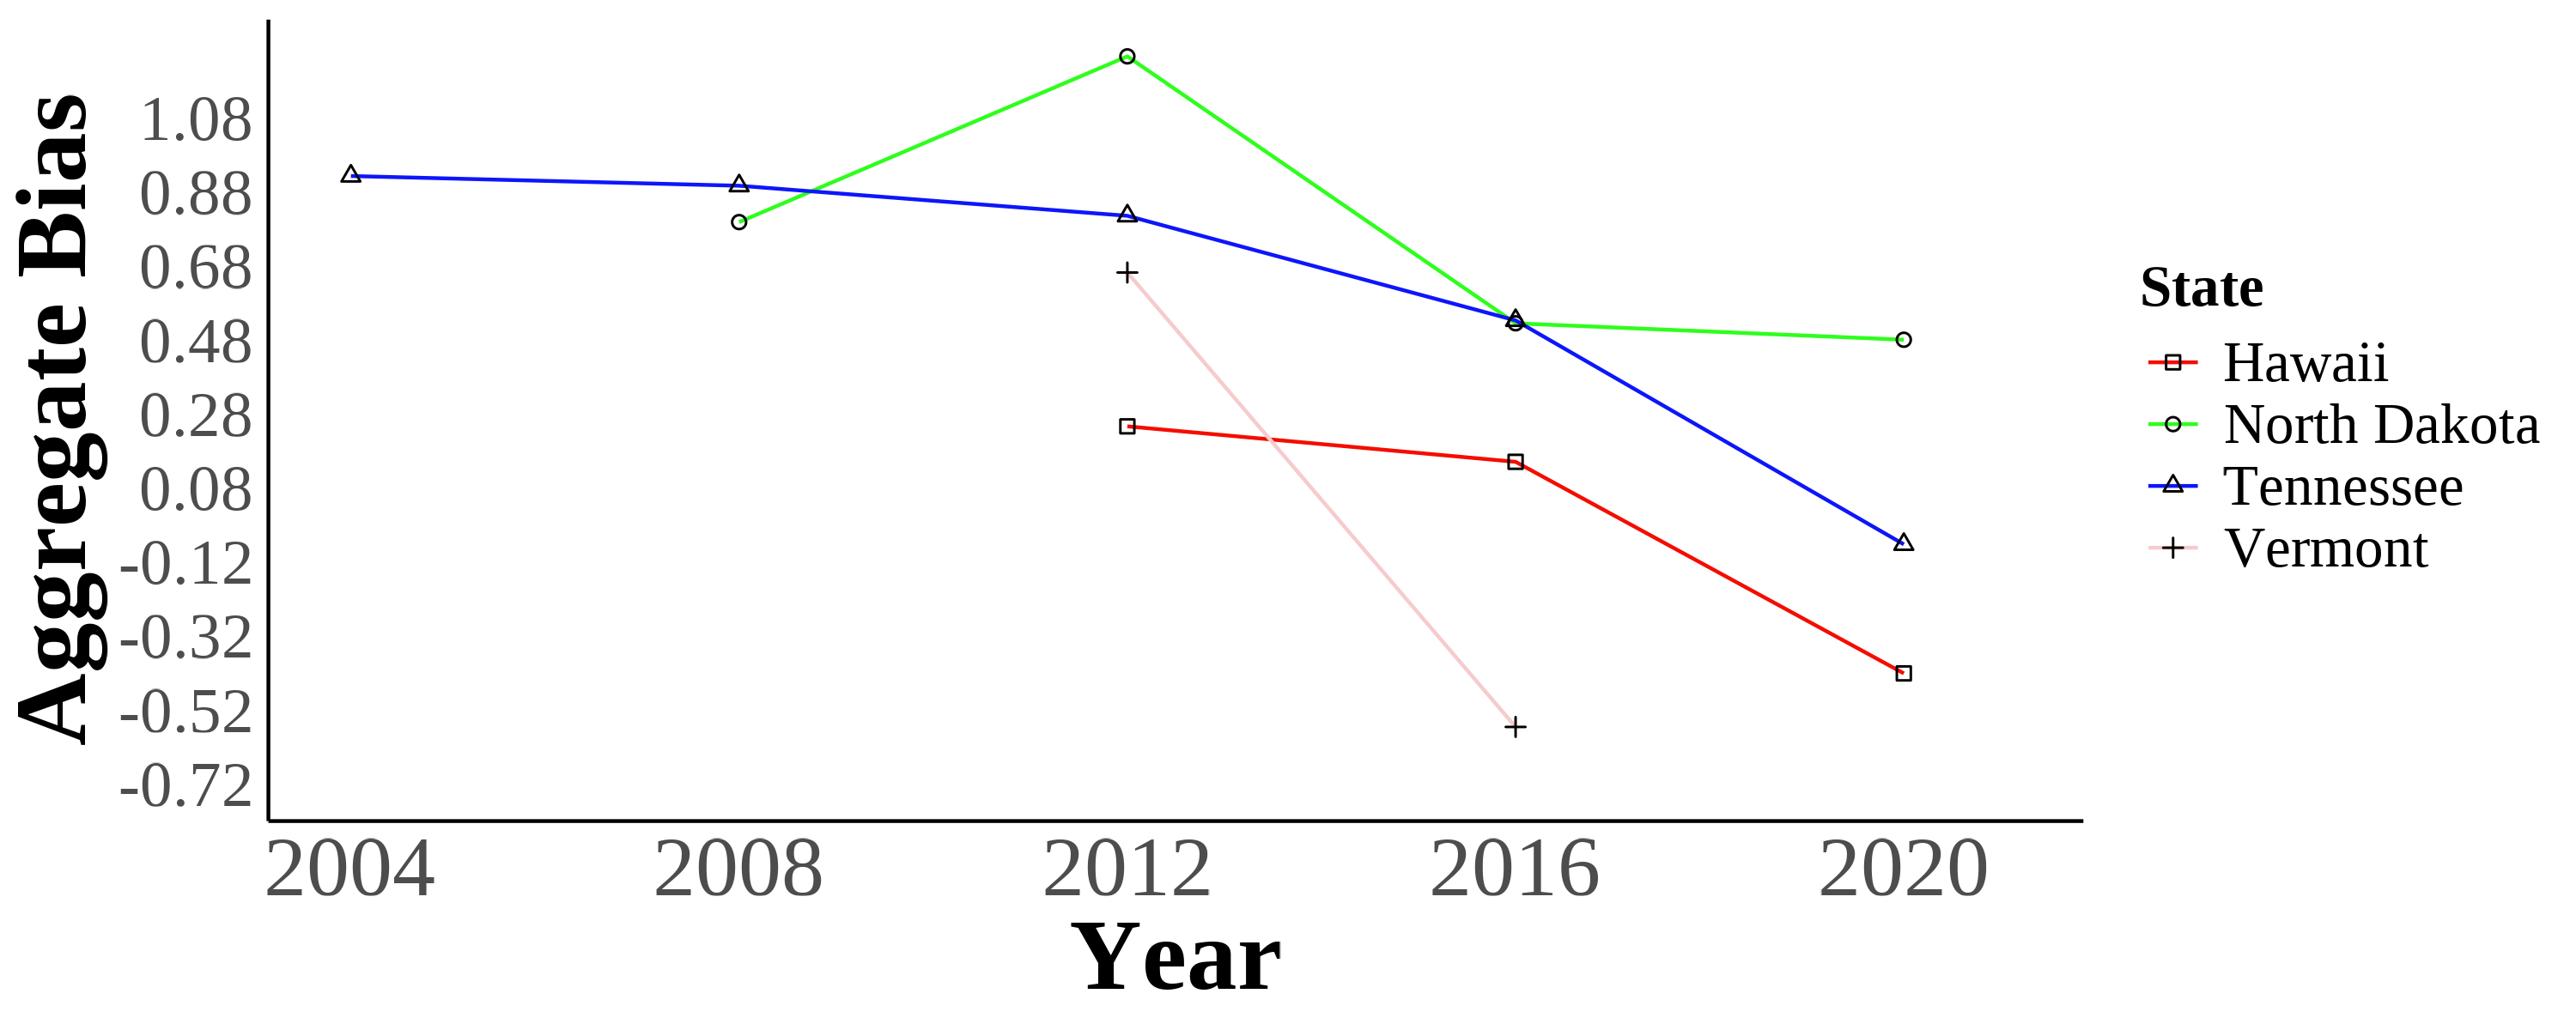
\includegraphics[width=.9\linewidth]{figure/Bias_twostates.png} 
\label{fig:skiniat}
\end{subfigure}
% Second
\begin{subfigure}{.9\textwidth}
\caption{Self-reported Asian Identity Over Time}
\centering
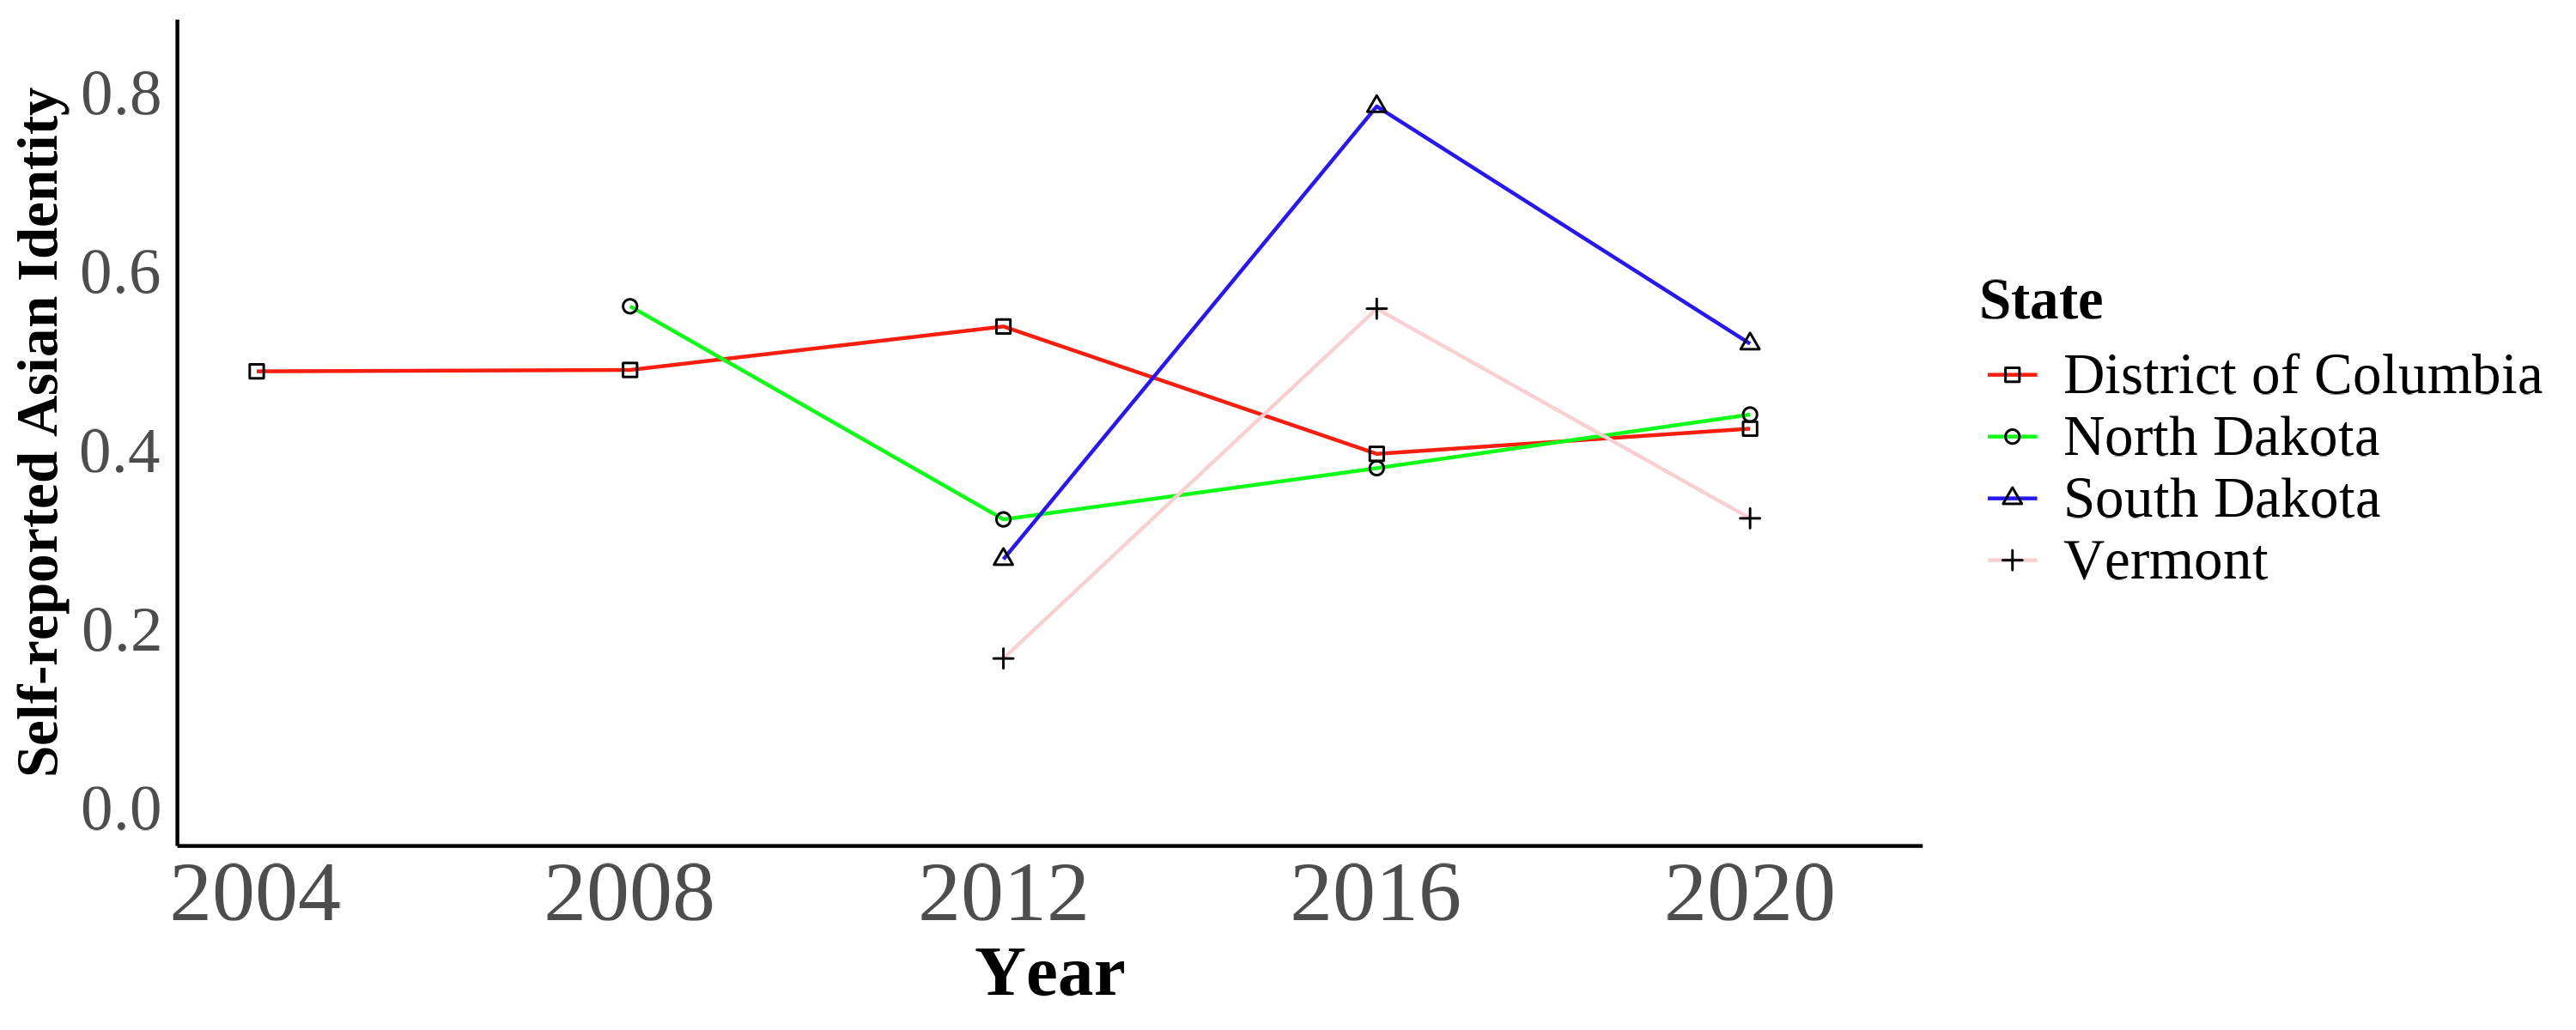
\includegraphics[width=.9\linewidth]{figure/Bias_twostates-asian.png} 
\label{fig:Asian-twostates}
\end{subfigure}
\caption*{\footnotesize{These two panels show the trends in implicit bias (panel a) and self-reported Asian identity among Asian immigrants (panel b) of the least and most biased places in the data. The District of Colombia is the least biased geographical area, and North Dakota is the most biased. The bias units are in standard deviations. Self-reported Asian identity is among first, second, and third-generation Asian immigrants aged 17 and younger still living in intact families.\\
Bias data is from the 2004-2021 Harvard's Project Implicit Association Test scores. Identity data is from the 2004-2021 Current Population Survey (CPS).}}
\end{figure}
\end{center}


\newpage
\pagebreak

\begin{center}
\begin{figure}[H]
\caption{Maps of State-level Implicit Association Test Bias Over Time Measure with Census Division Regional Boundaries}
\label{fig:skiniat-maps}
% first
\begin{subfigure}{.45\textwidth}
\caption{State-level Bias in 2004}
\centering
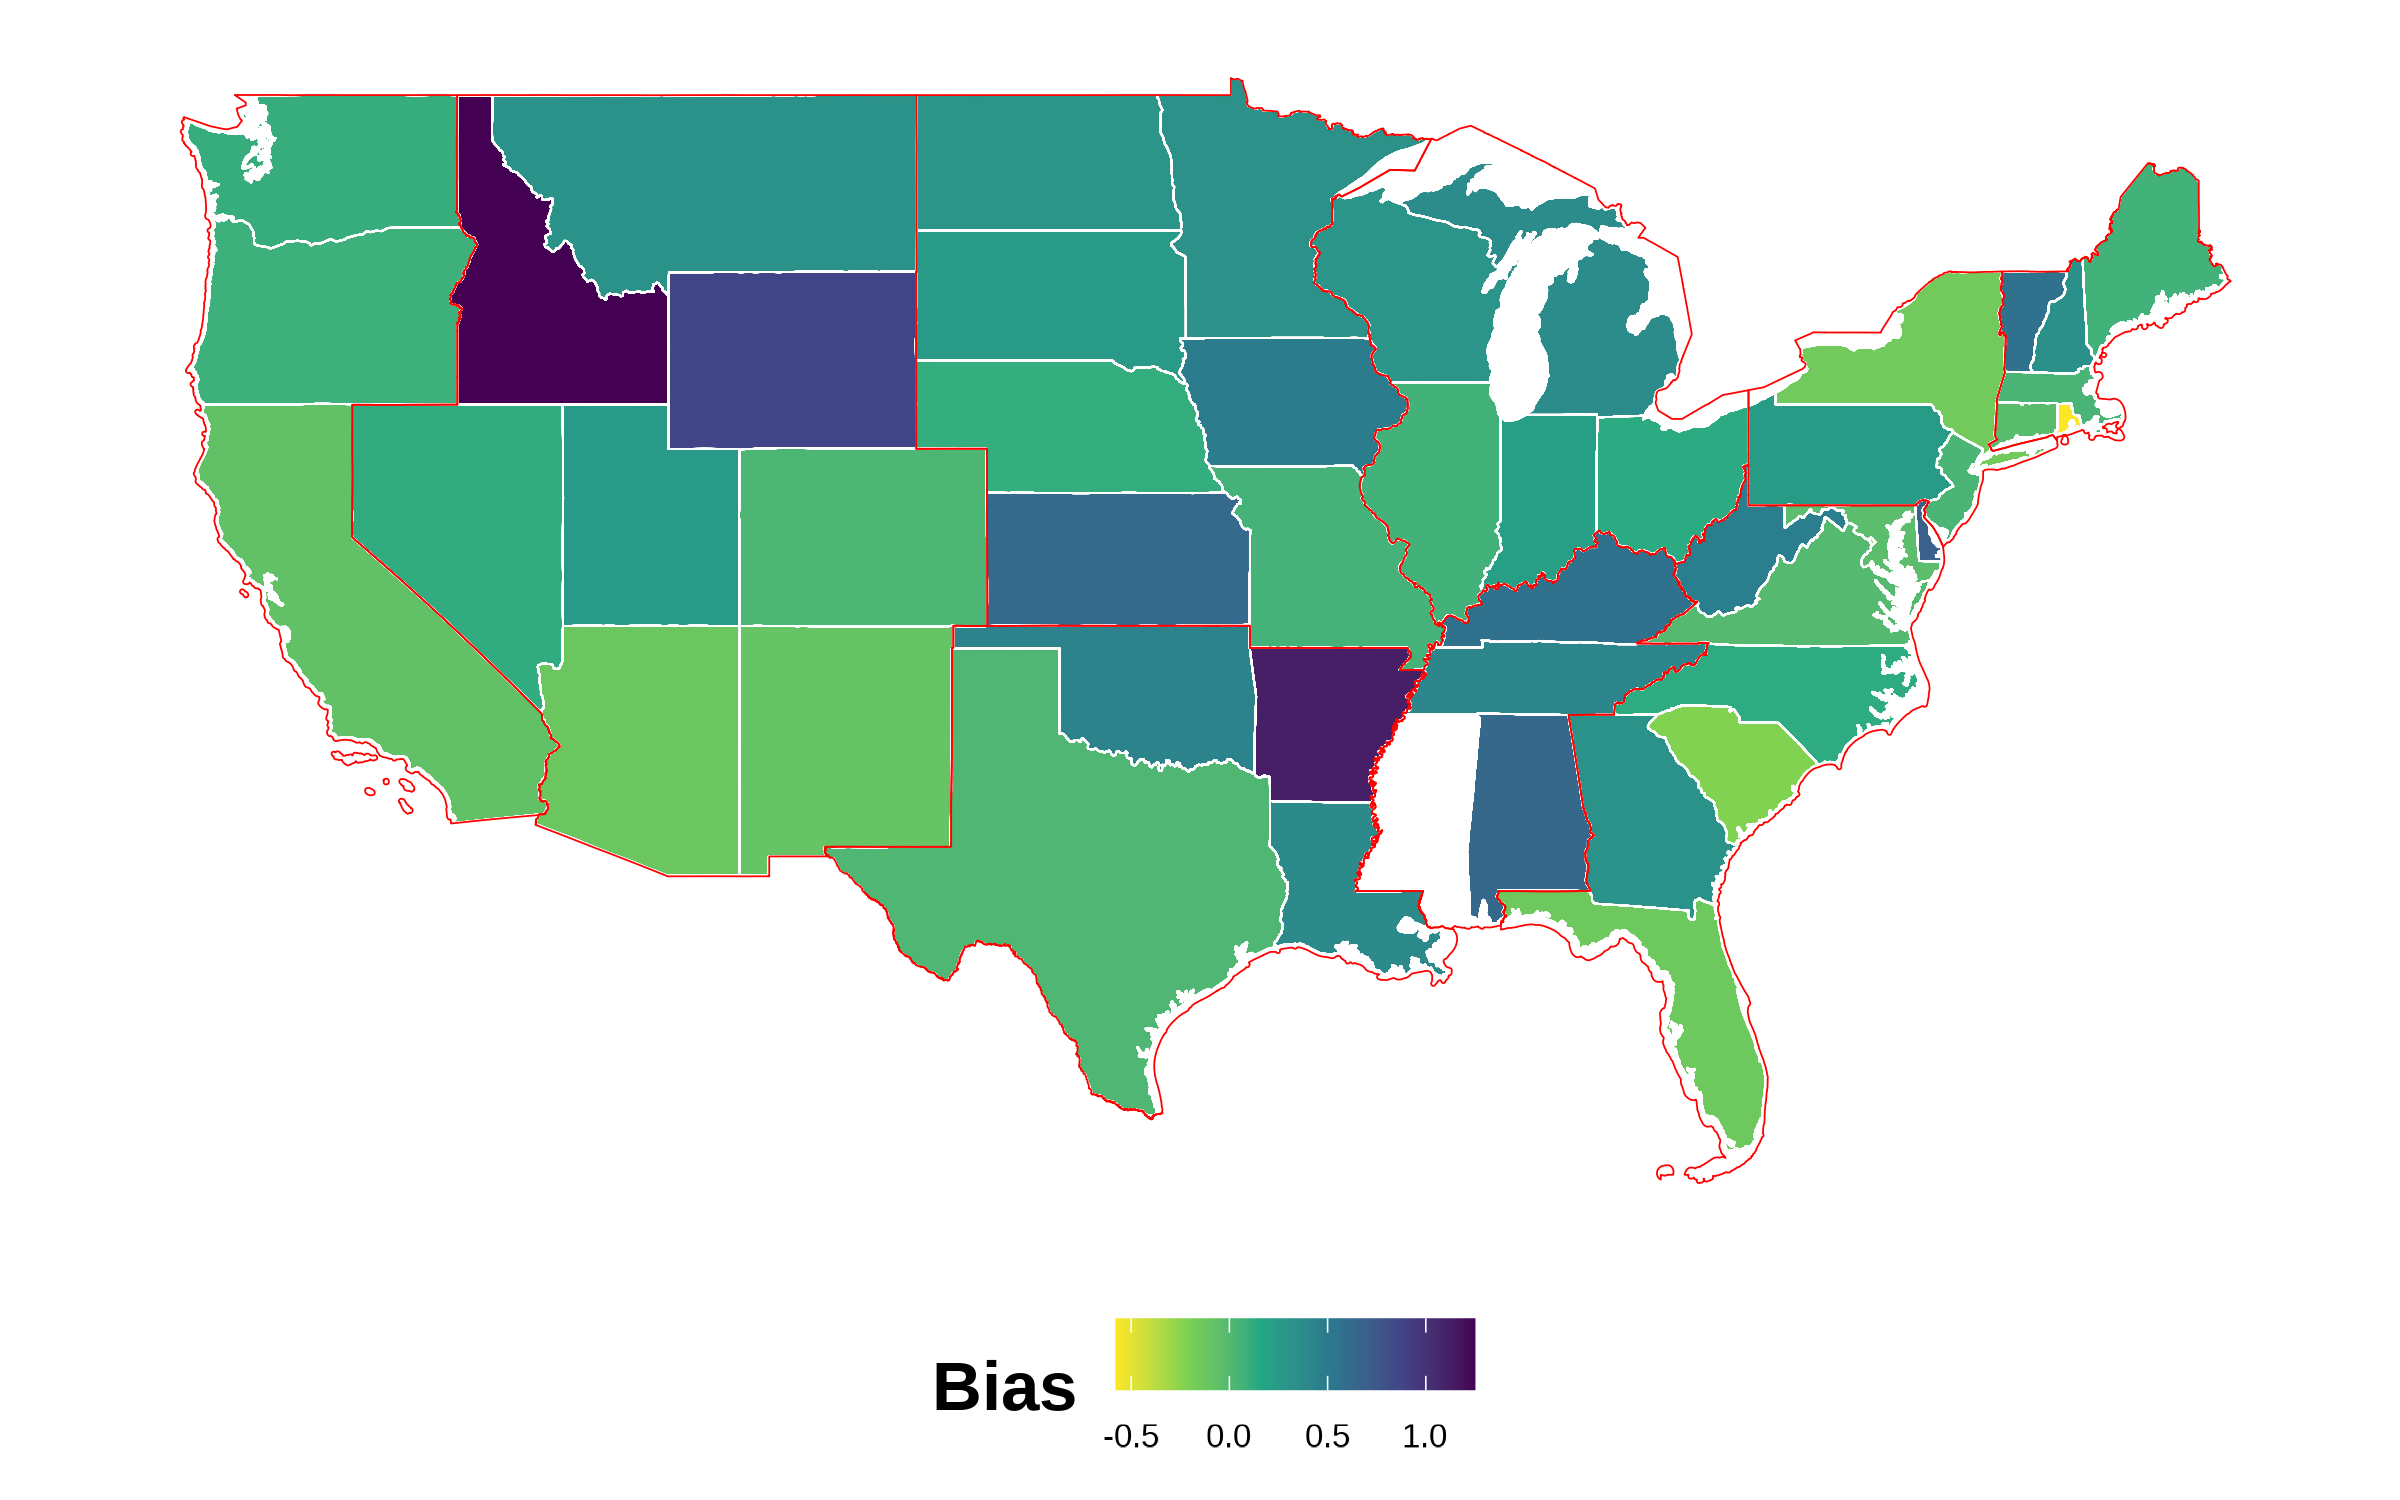
\includegraphics[width=0.9\linewidth]{figure/2004skinmap.png} 
\label{fig:skiniat-map-2004}
\end{subfigure}
\hfill%
% Second
\begin{subfigure}{.45\textwidth}
\caption{State-level Bias in 2006}
\centering
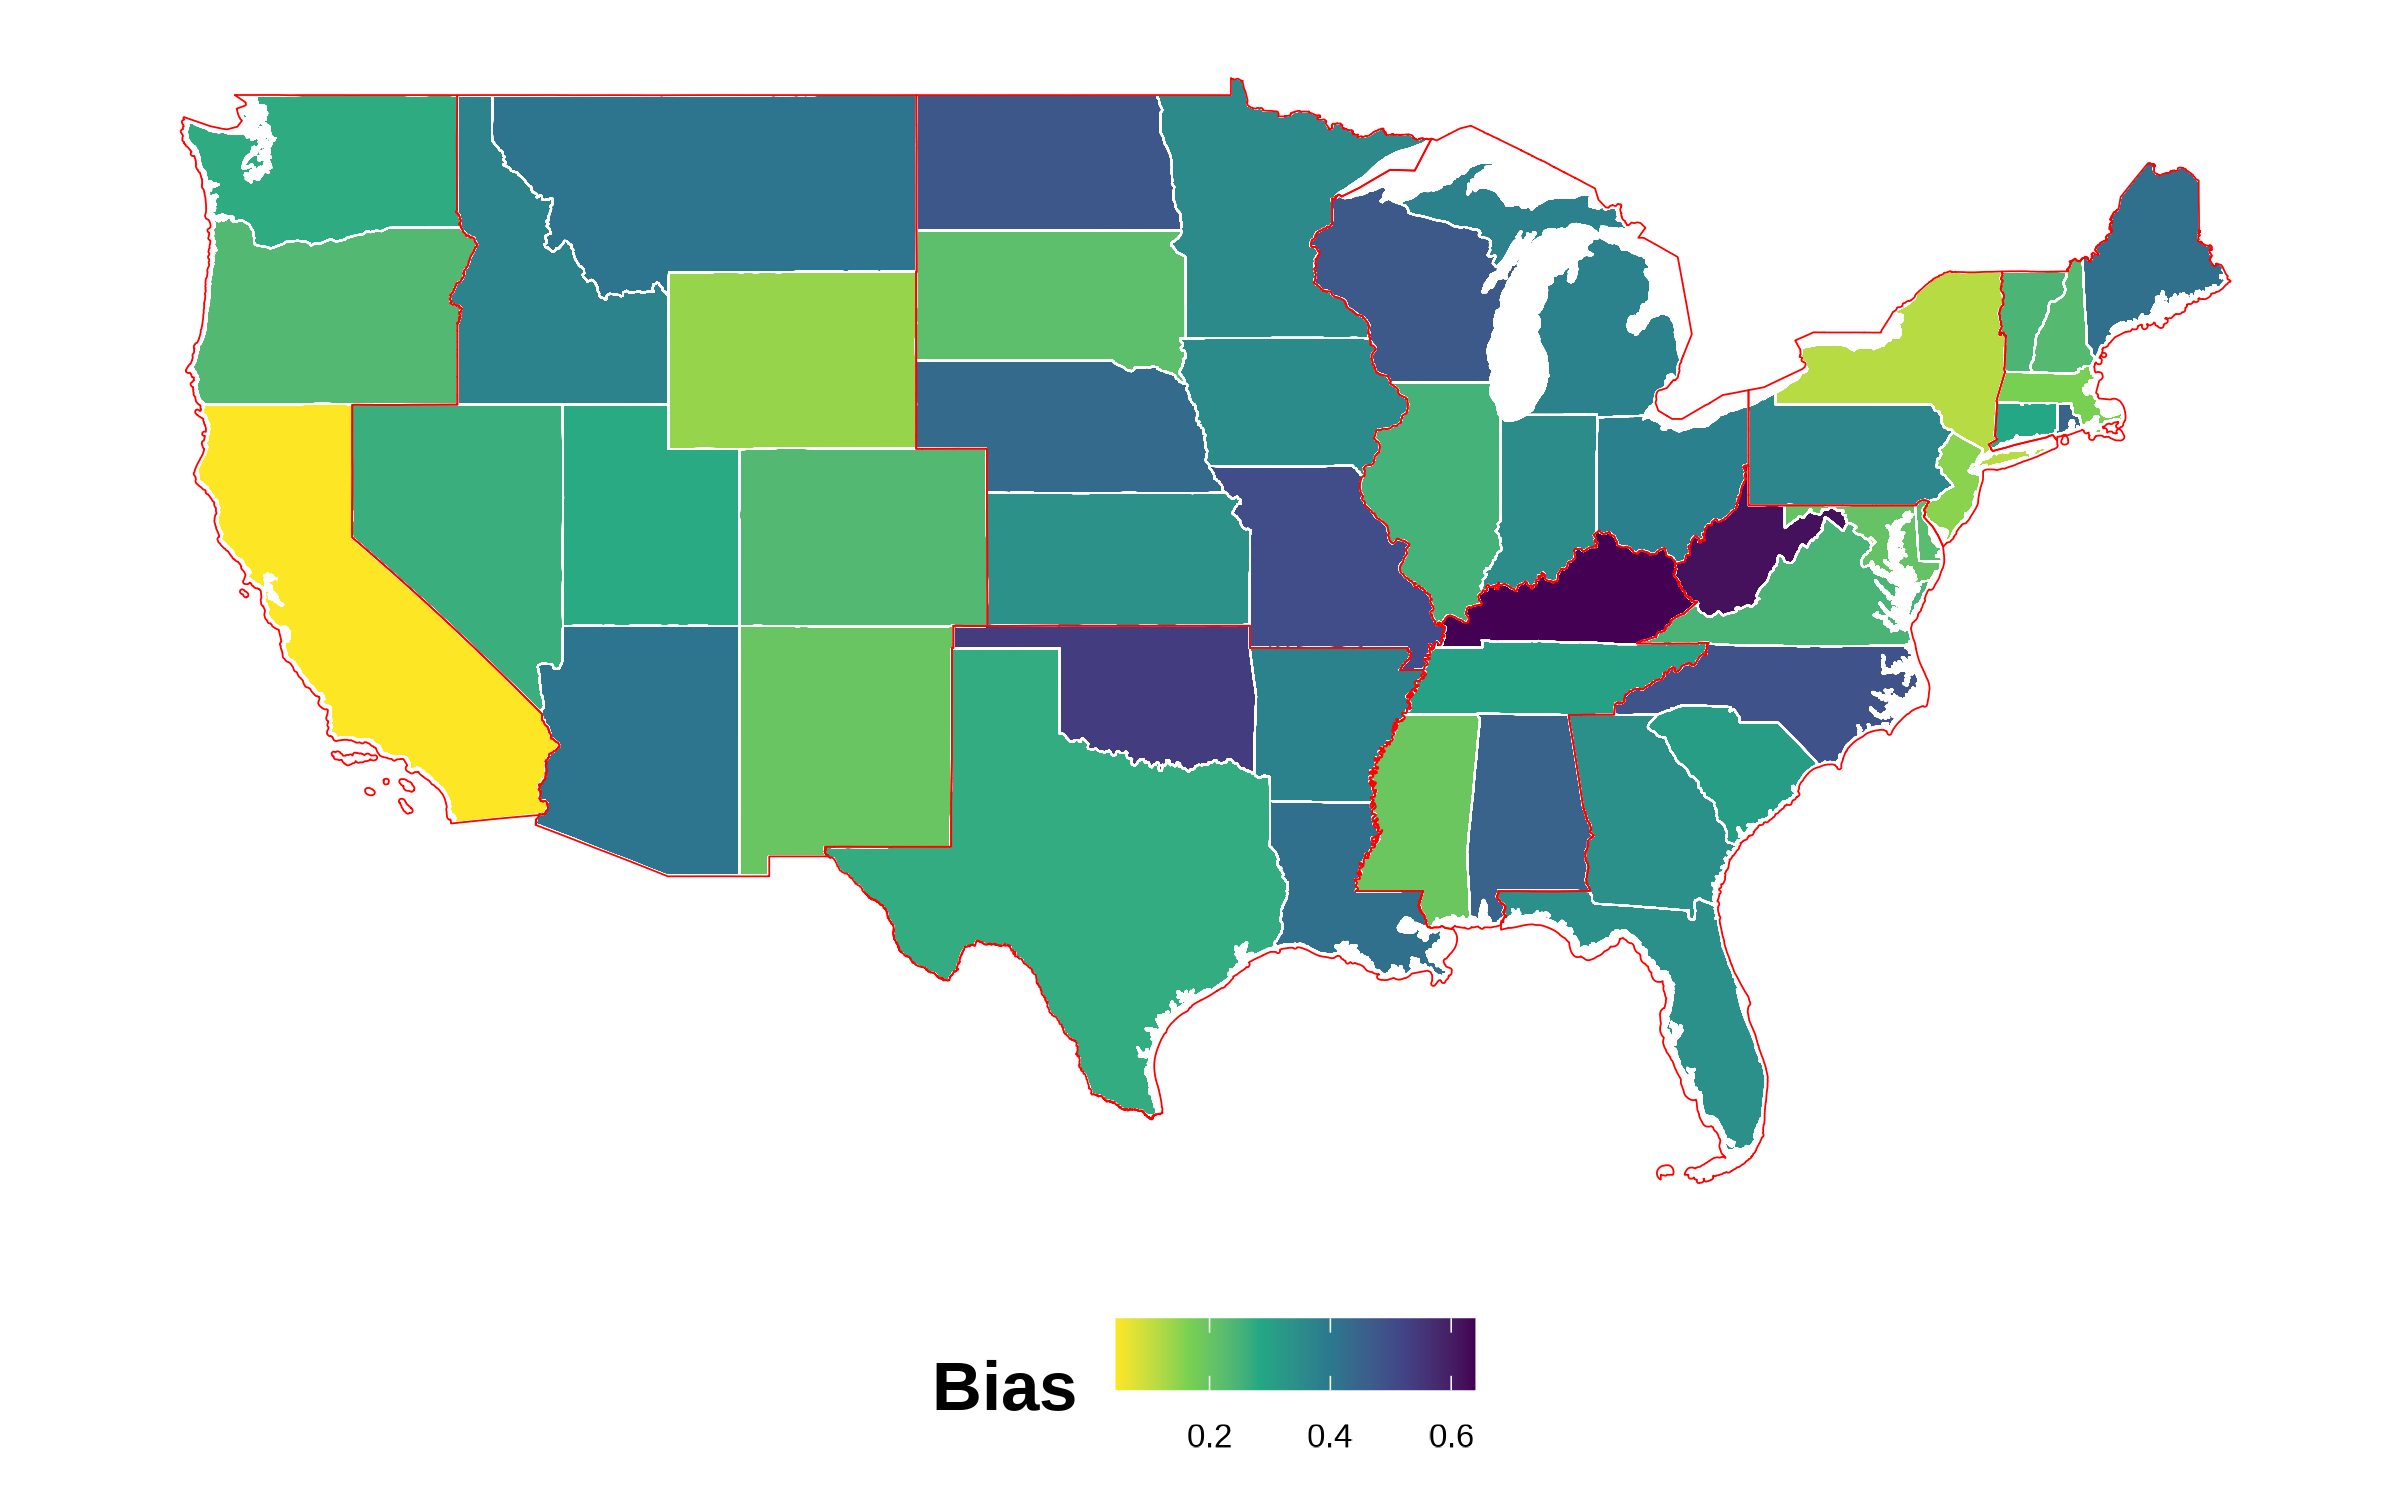
\includegraphics[width=0.9\linewidth]{figure/2006skinmap.png} 
\label{fig:skiniat-map-2006}
\end{subfigure}
\hfill%
% third
\begin{subfigure}{.45\textwidth}
\caption{State-level Bias in 2008}
\centering
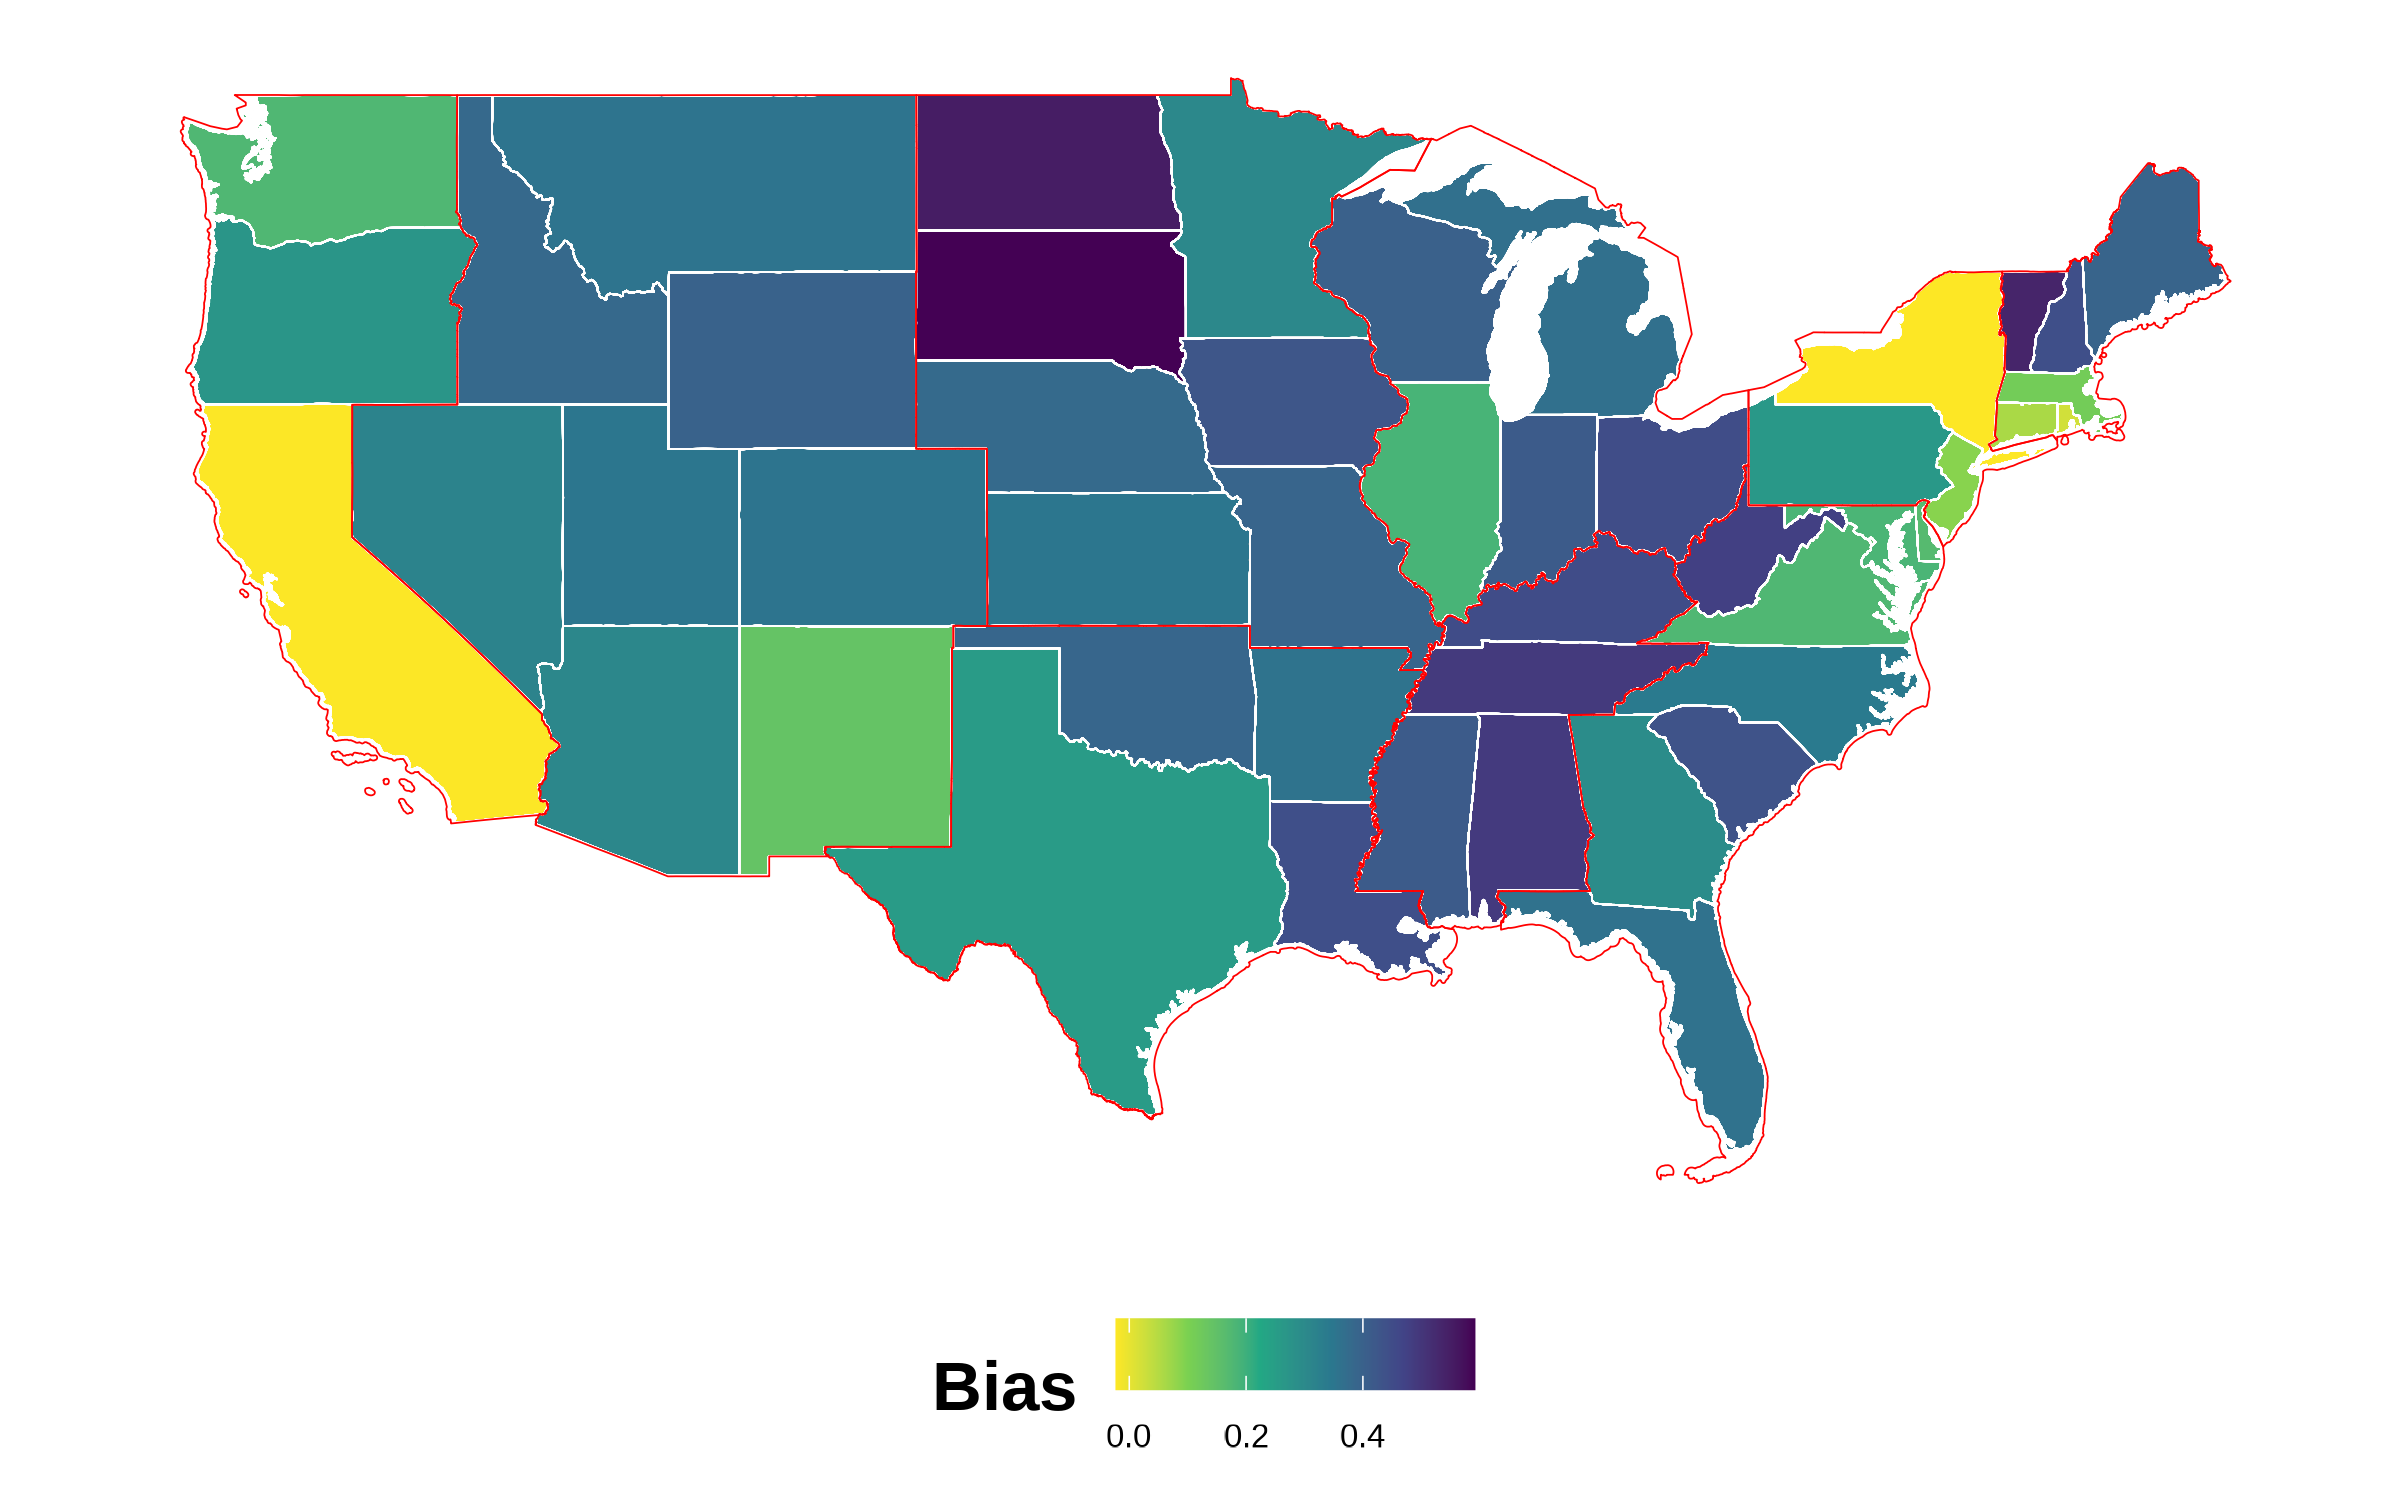
\includegraphics[width=0.9\linewidth]{figure/2008skinmap.png} 
\label{fig:skiniat-map-2008}
\end{subfigure}
\hfill%
% fourth
\begin{subfigure}{.45\textwidth}
\caption{State-level Bias in 2010}
\centering
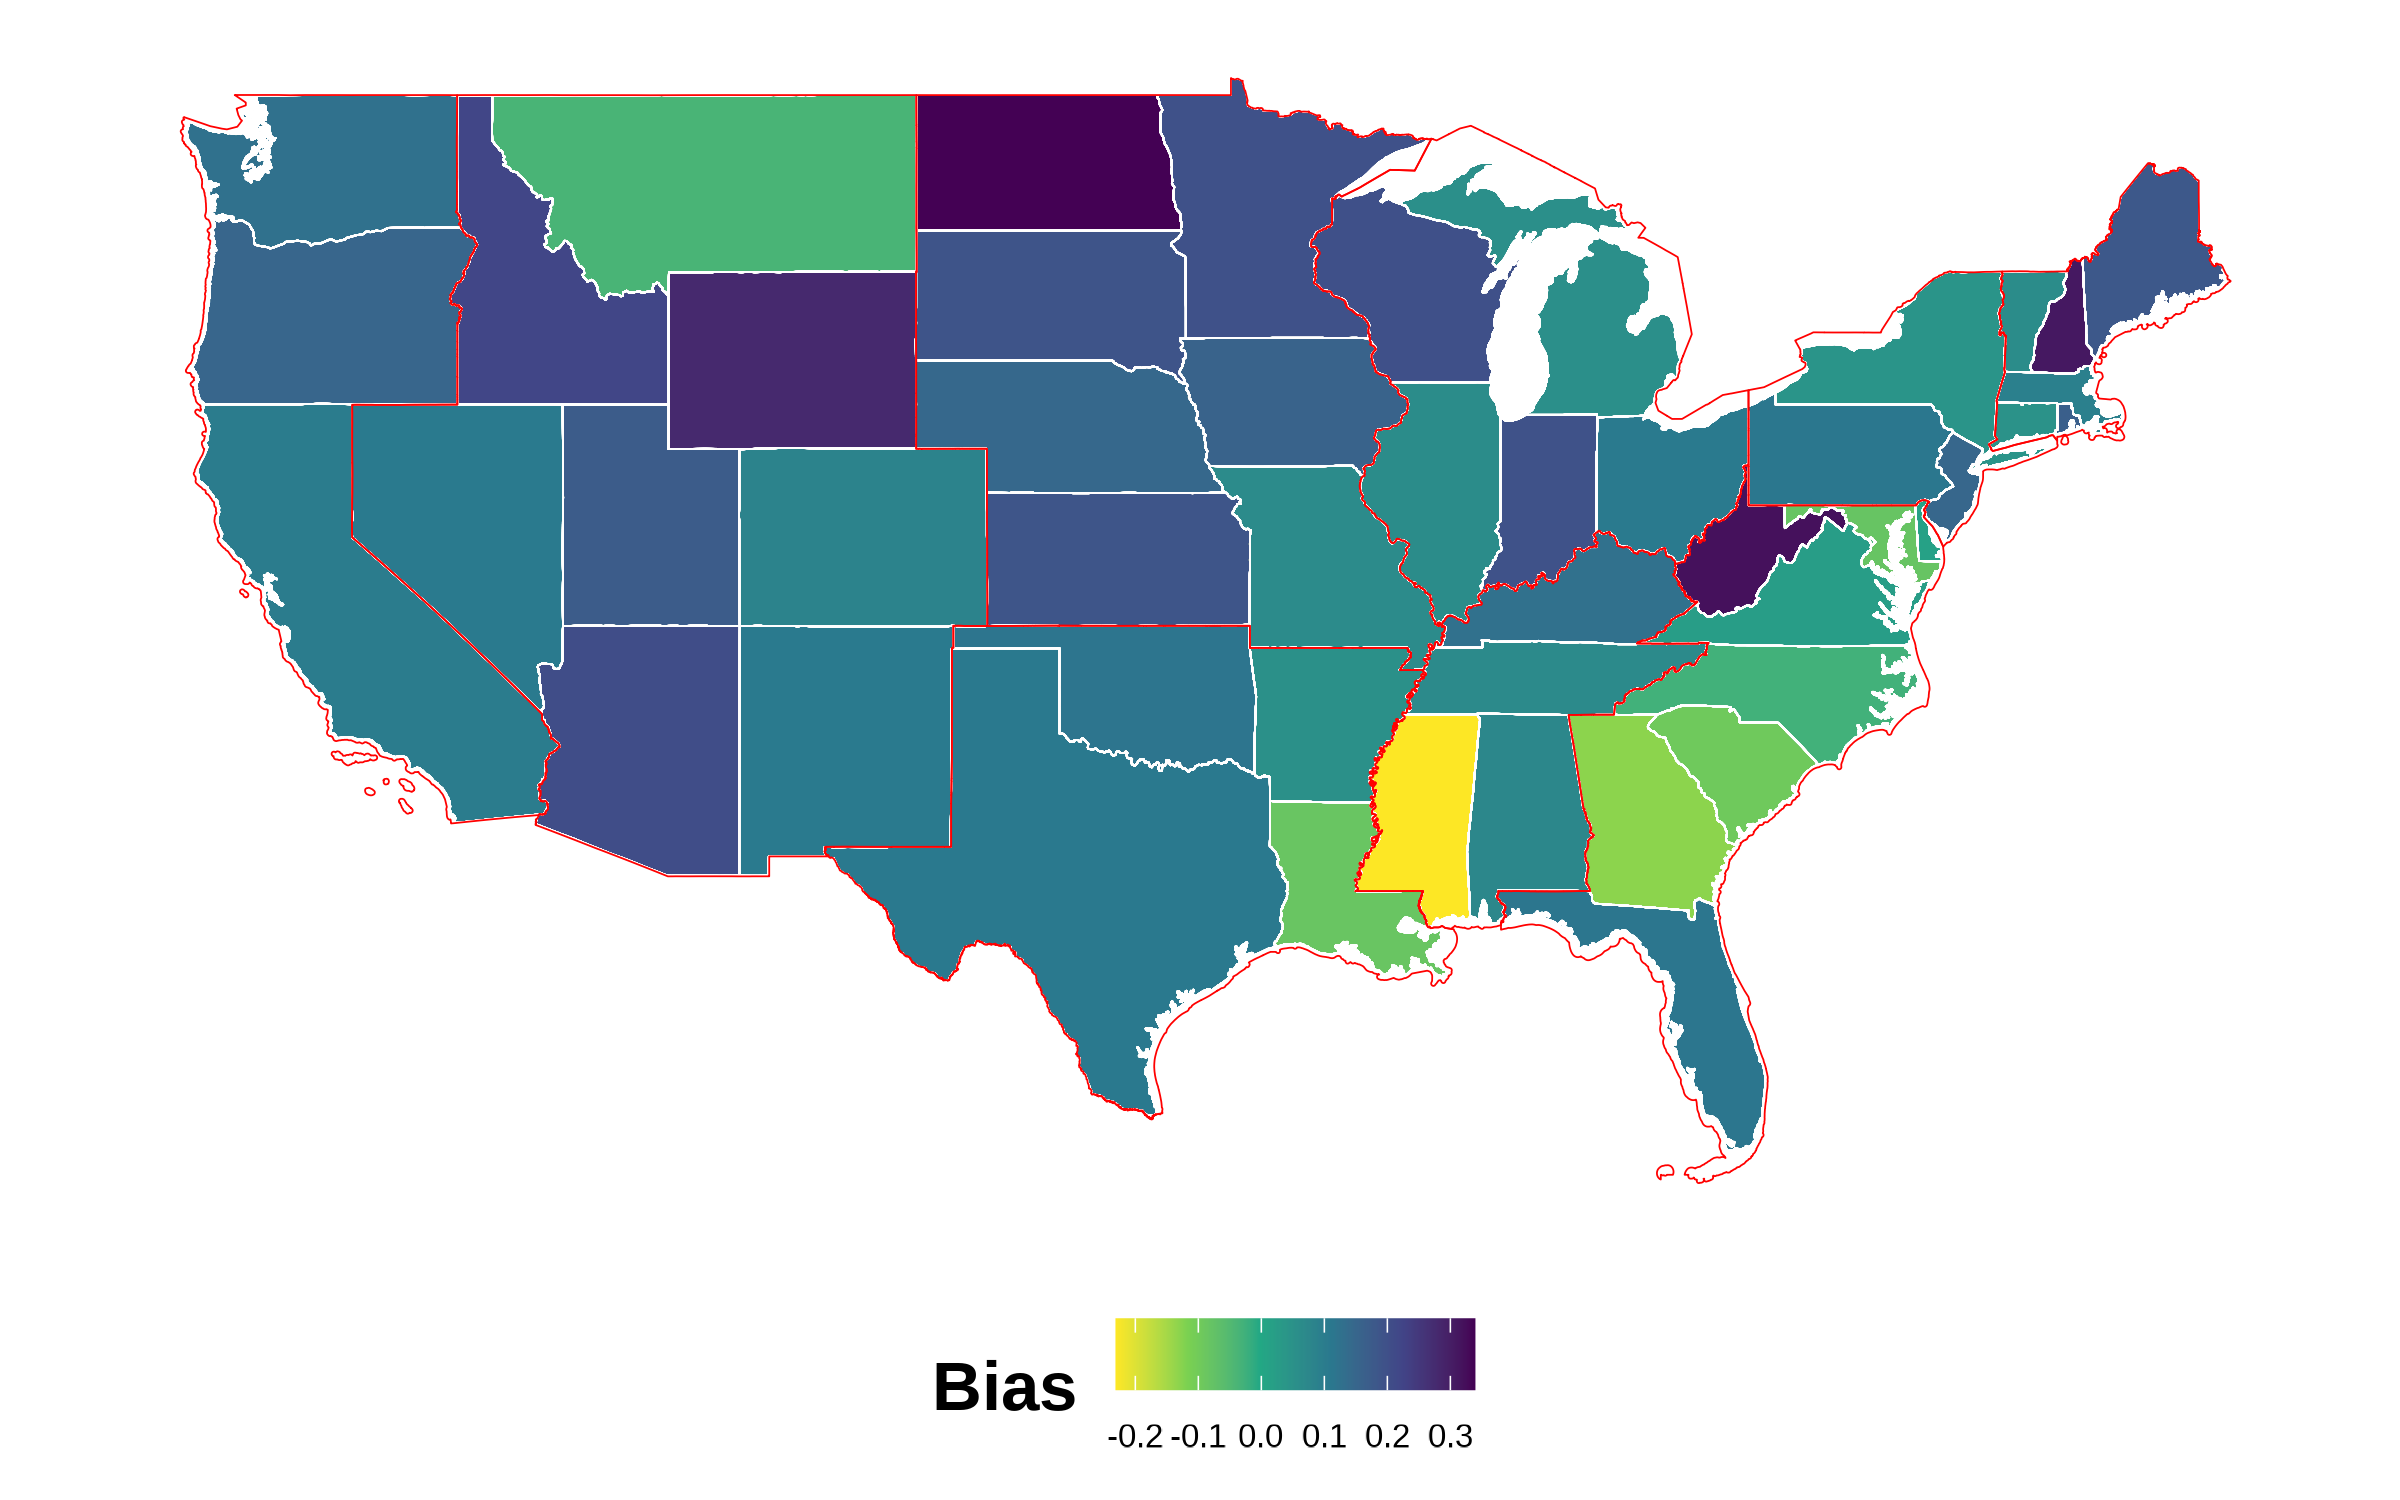
\includegraphics[width=0.9\linewidth]{figure/2010skinmap.png} 
\label{fig:skiniat-map-2010}
\end{subfigure}
\hfill%
% fifth
\begin{subfigure}{.45\textwidth}
\caption{State-level Bias in 2012}
\centering
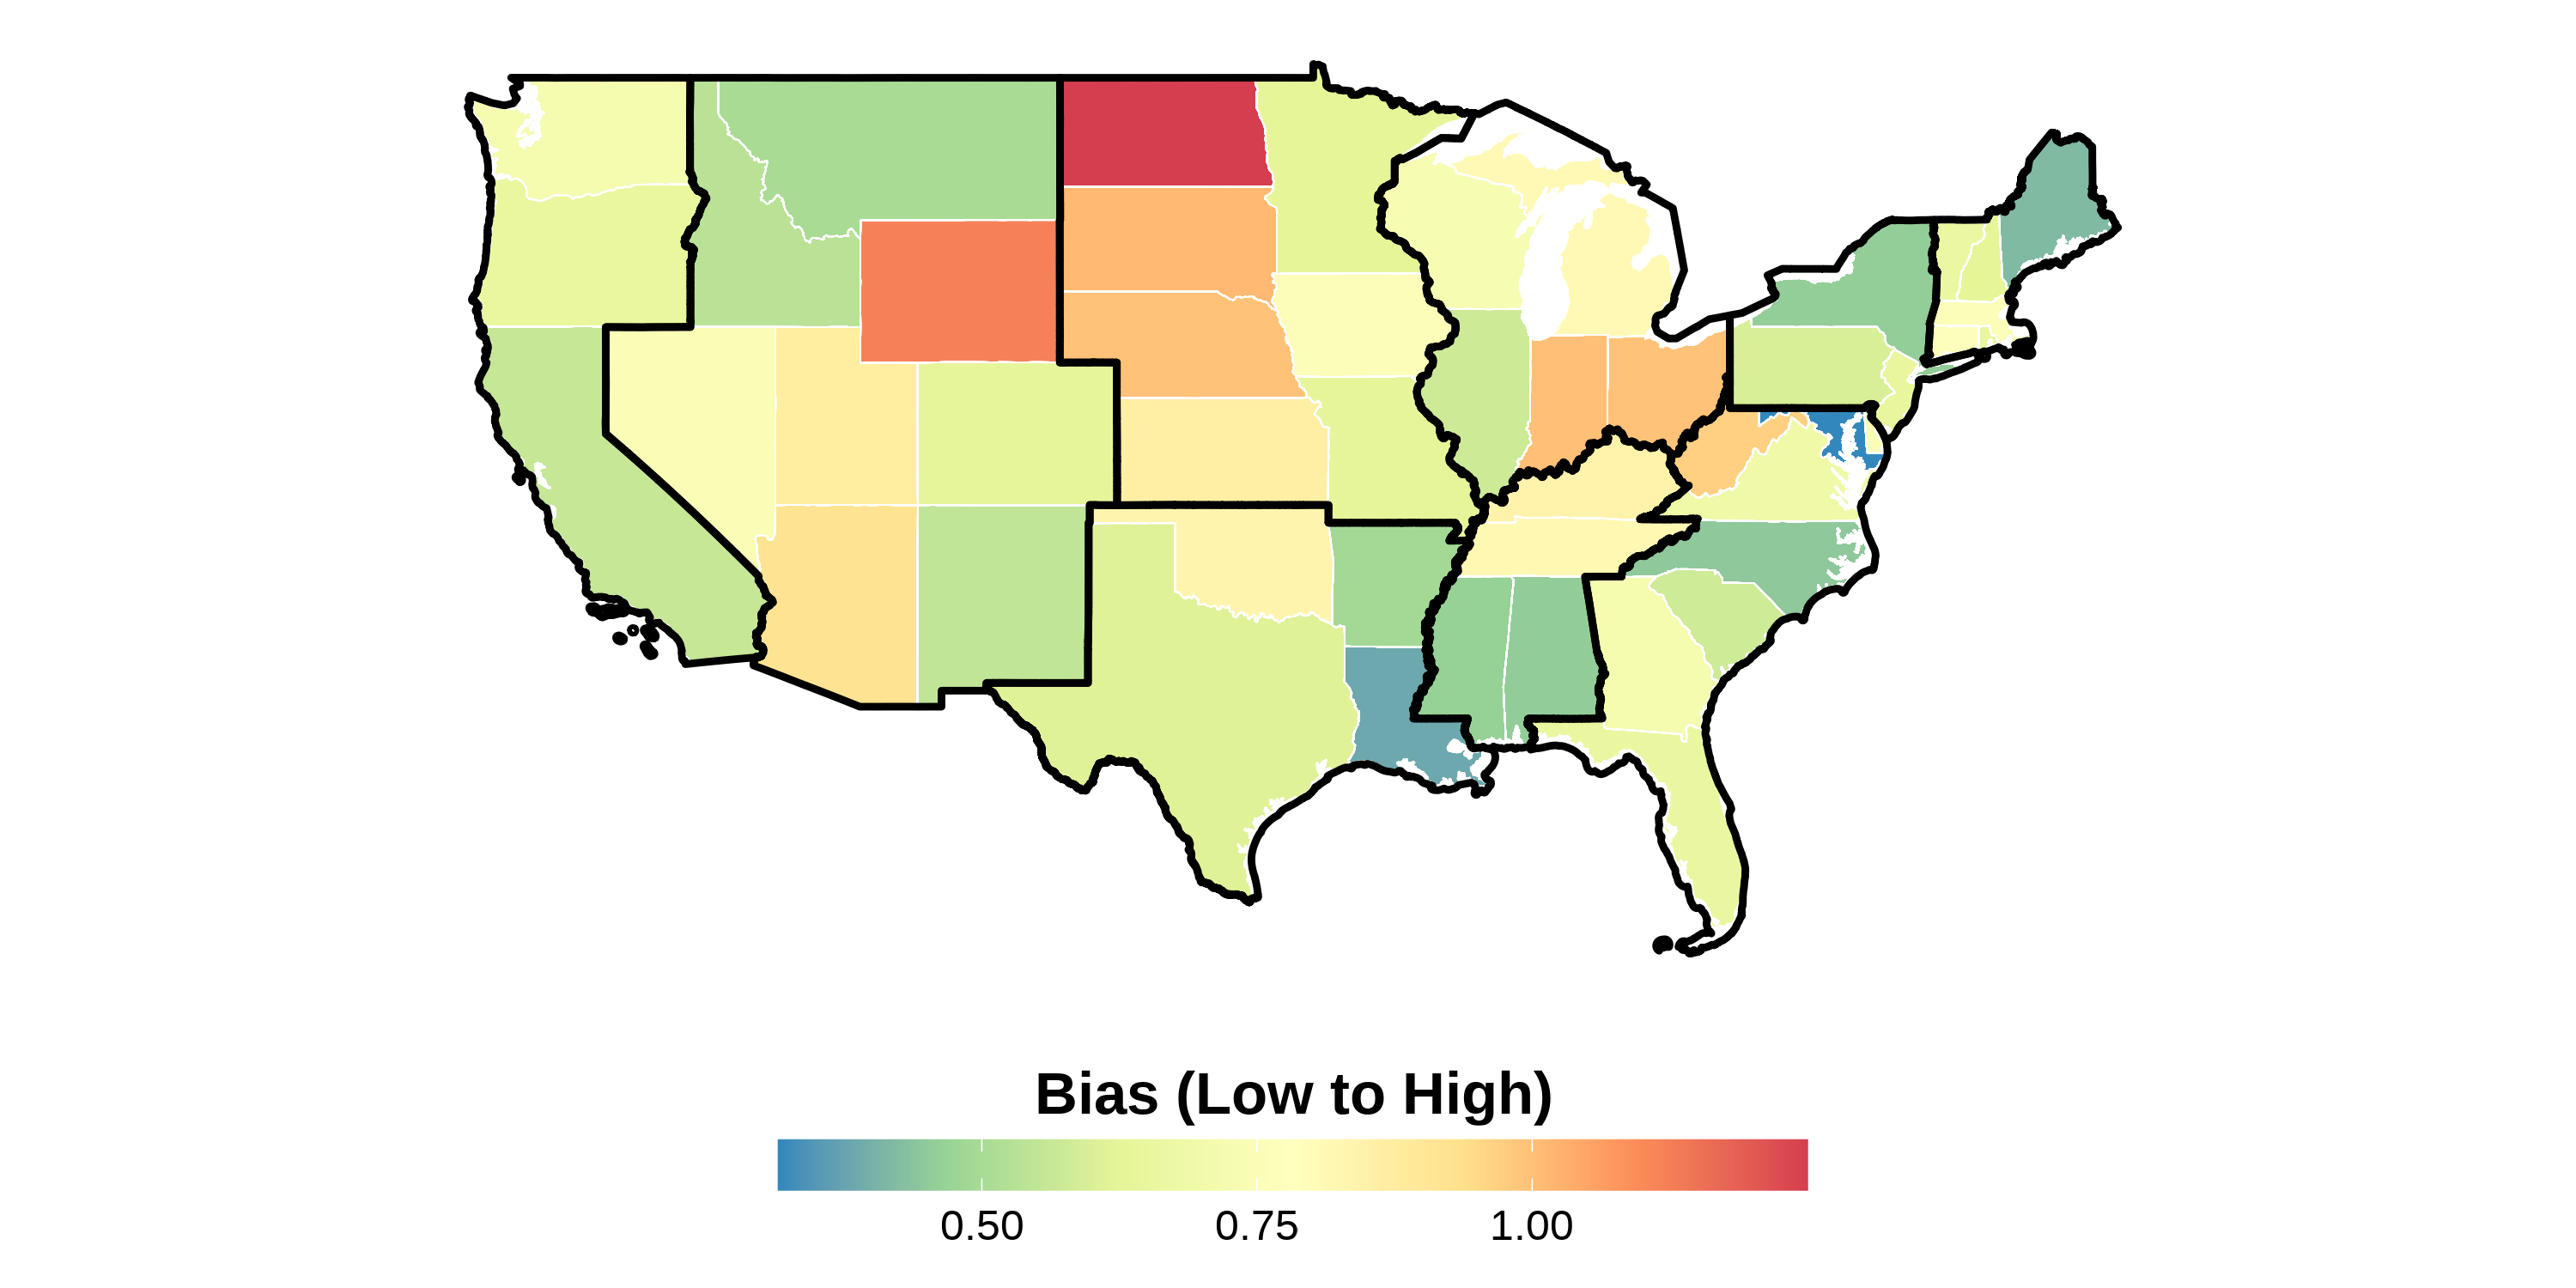
\includegraphics[width=0.9\linewidth]{figure/2012skinmap.png} 
\label{fig:skiniat-map-2012}
\end{subfigure}
\hfill%
% sixth
\begin{subfigure}{.45\textwidth}
\caption{State-level Bias in 2014}
\centering
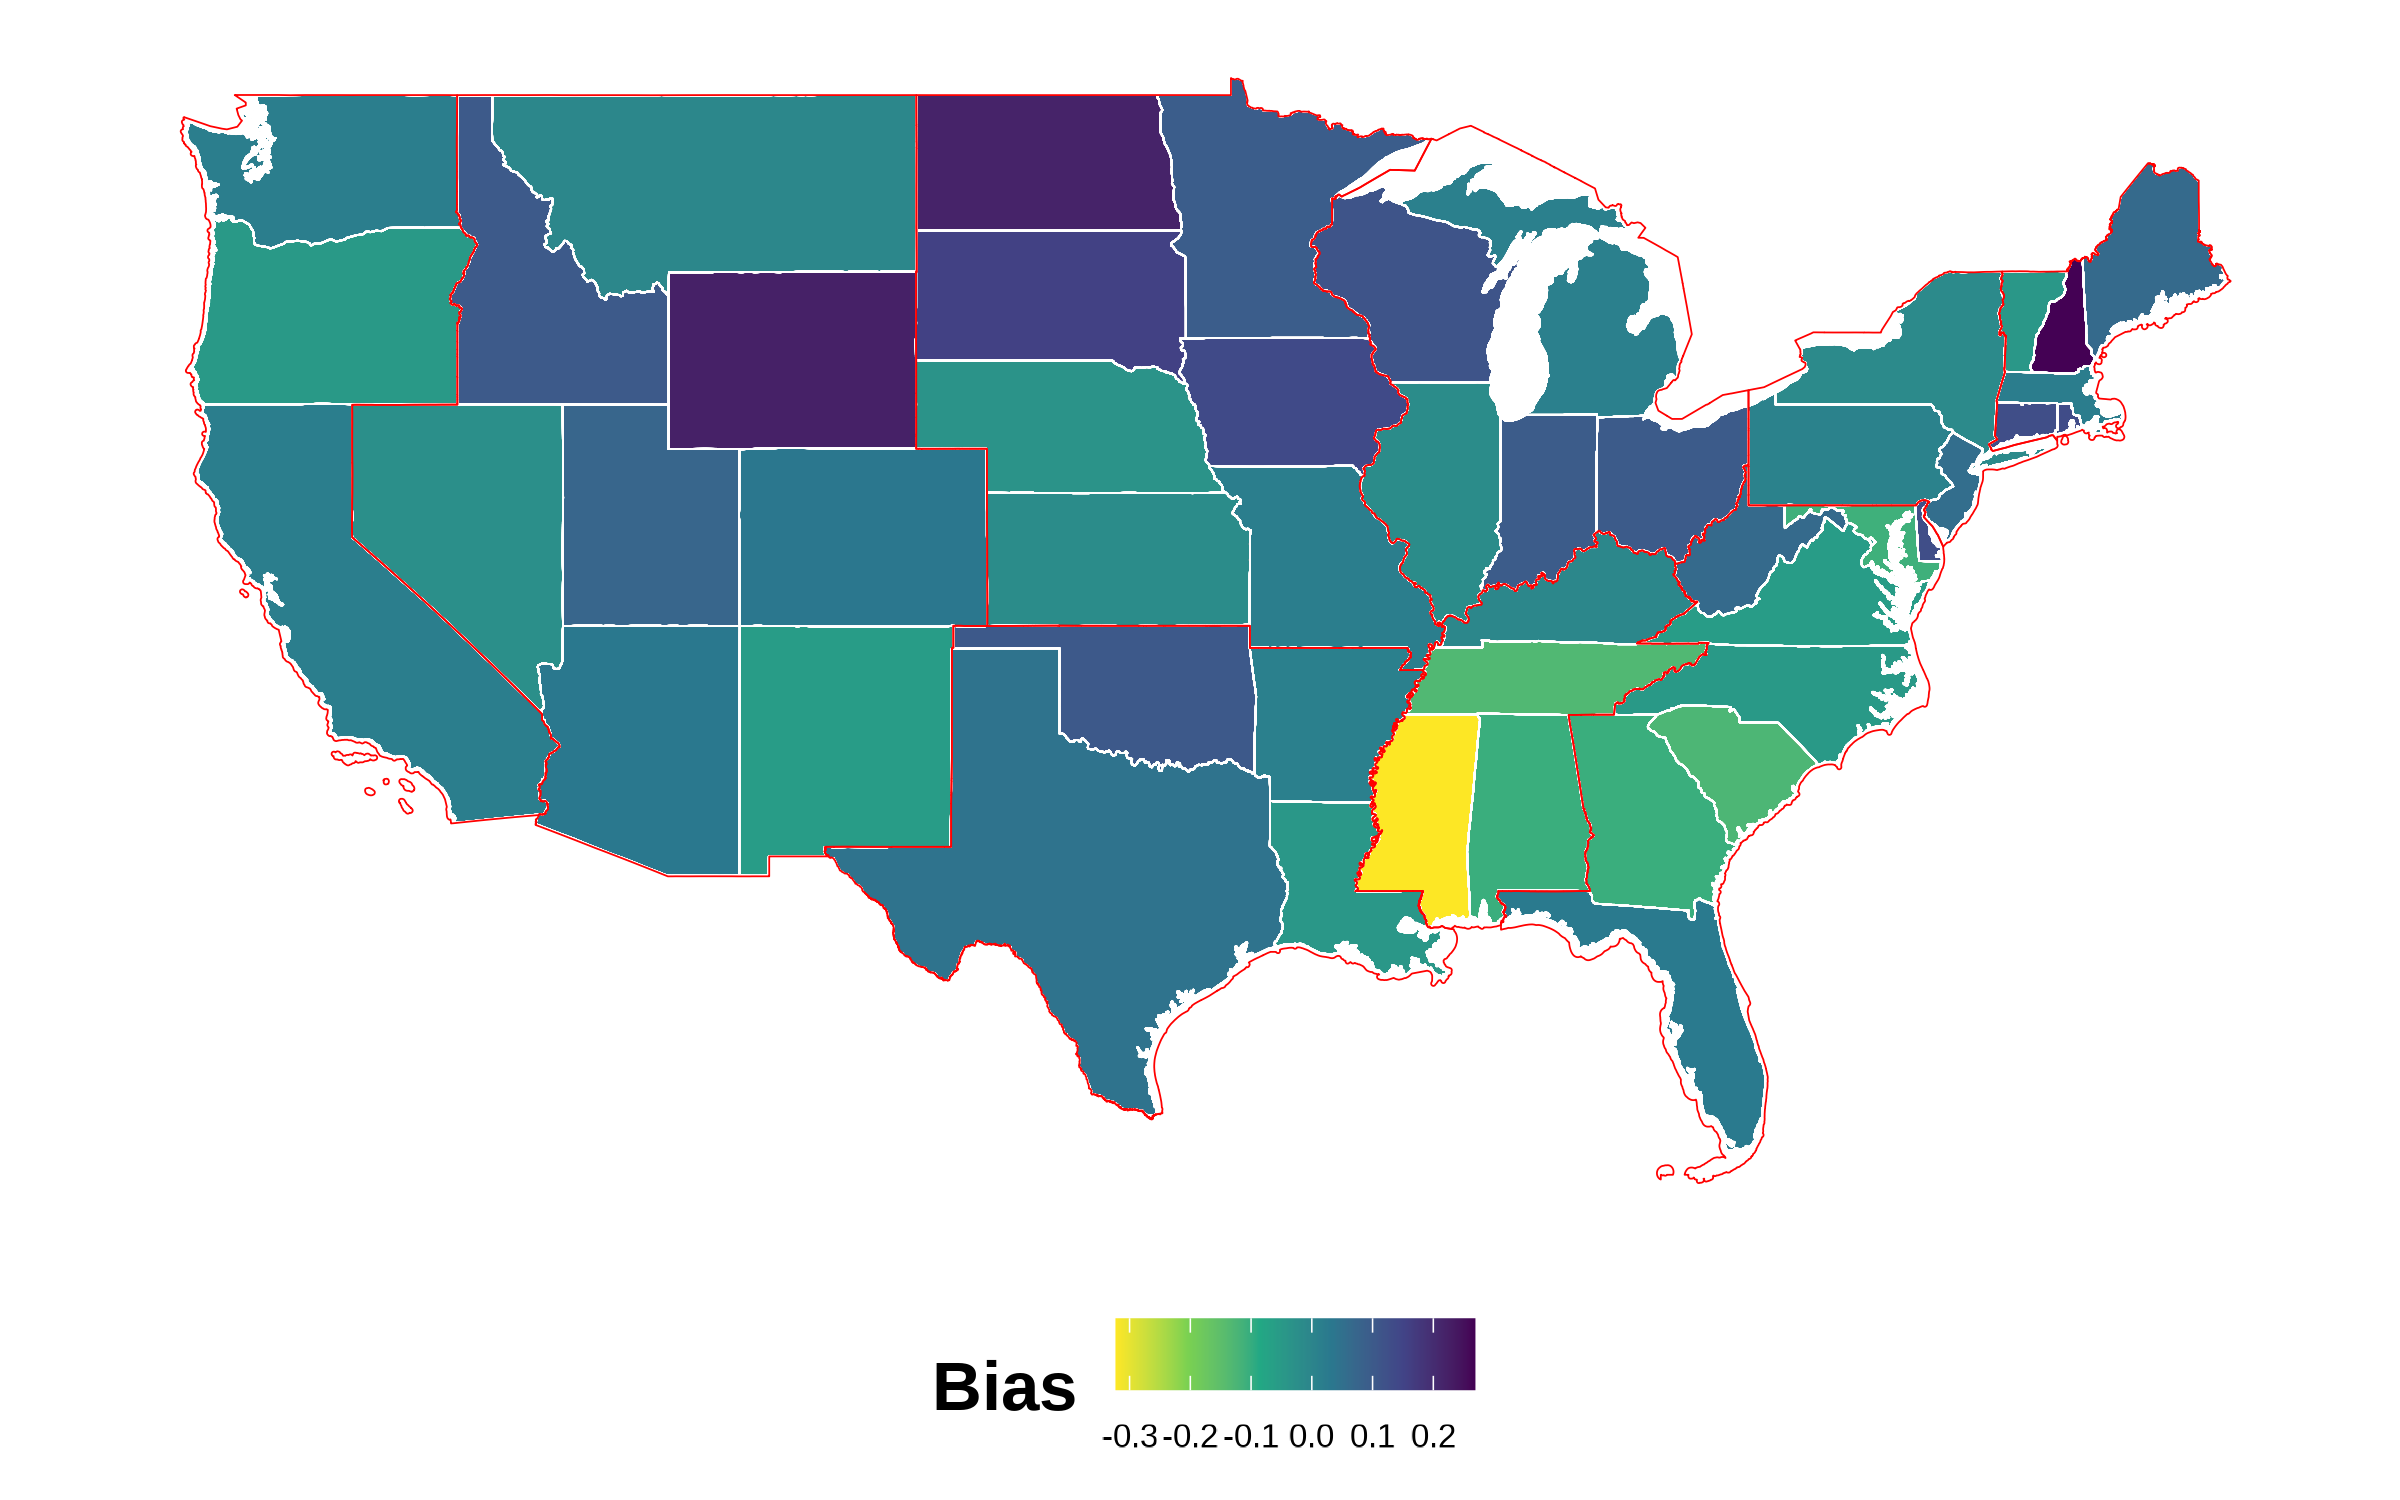
\includegraphics[width=0.9\linewidth]{figure/2014skinmap.png} 
\label{fig:skiniat-map-2014}
\end{subfigure}
\hfill%
% seventh
\begin{subfigure}{.45\textwidth}
\caption{State-level Bias in 2016}
\centering
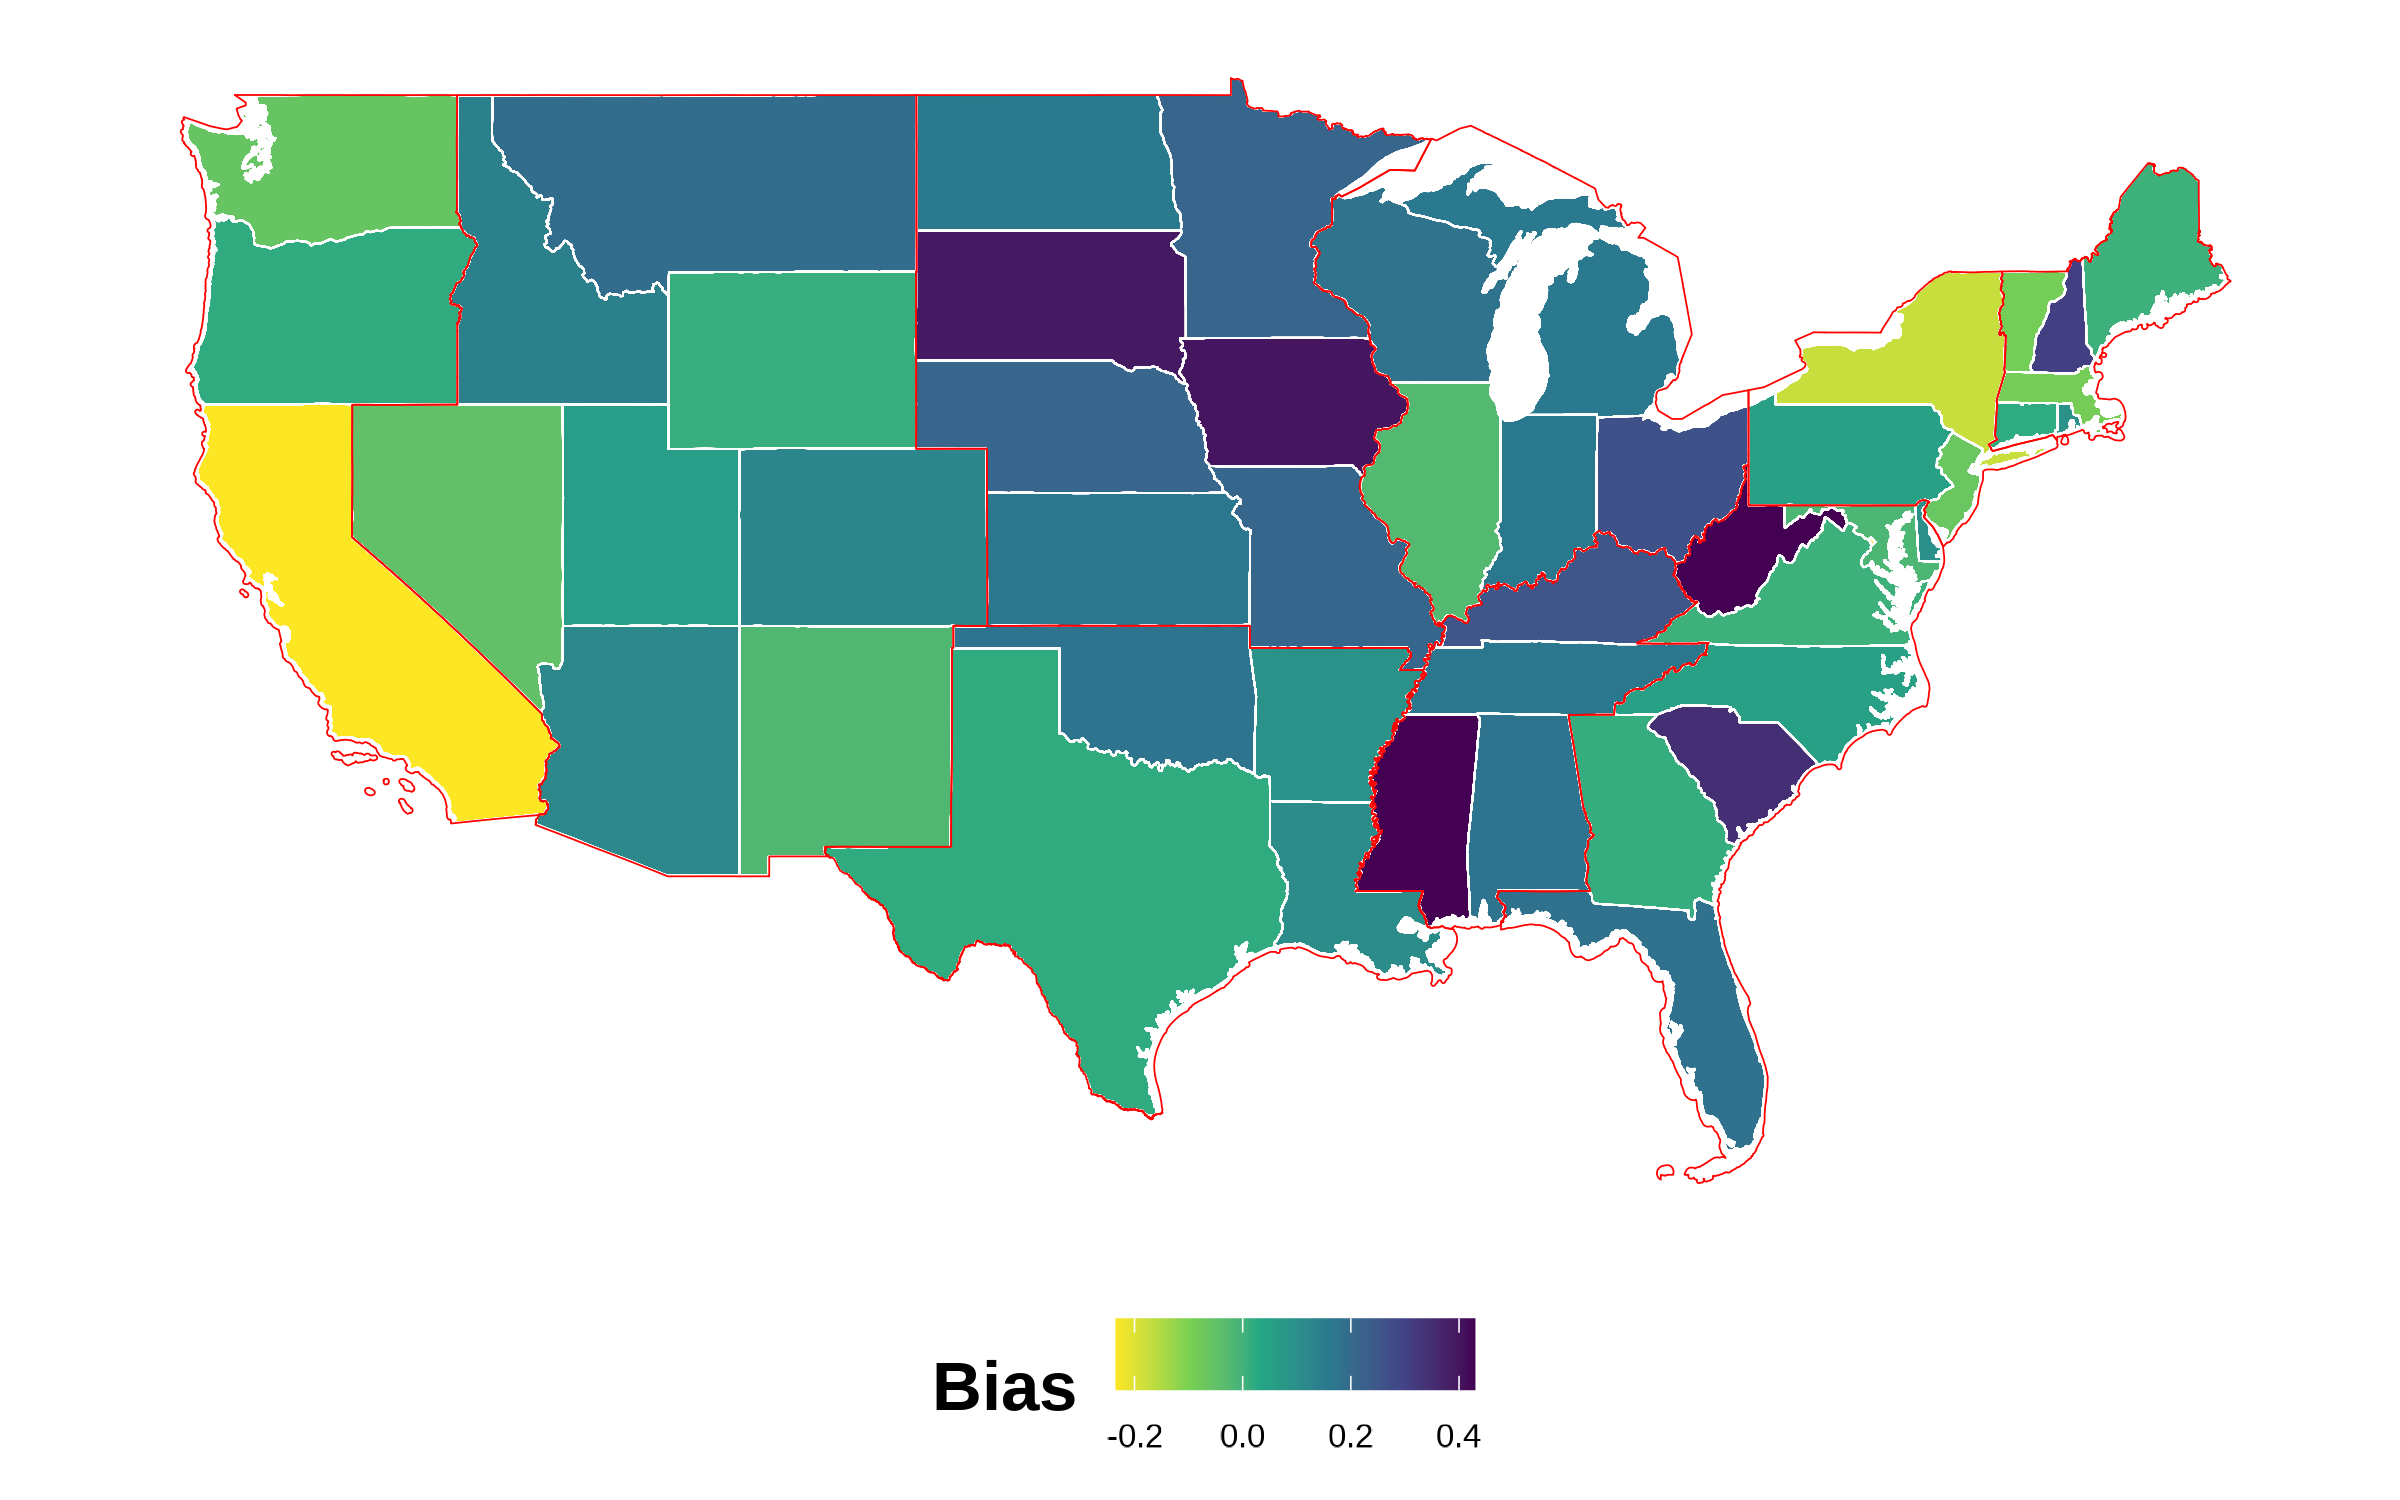
\includegraphics[width=0.9\linewidth]{figure/2016skinmap.png} 
\label{fig:skiniat-map-2016}
\end{subfigure}
\hfill%
% eigth
\begin{subfigure}{.45\textwidth}
\hspace{1cm}
\caption{State-level Bias in 2018}
\centering
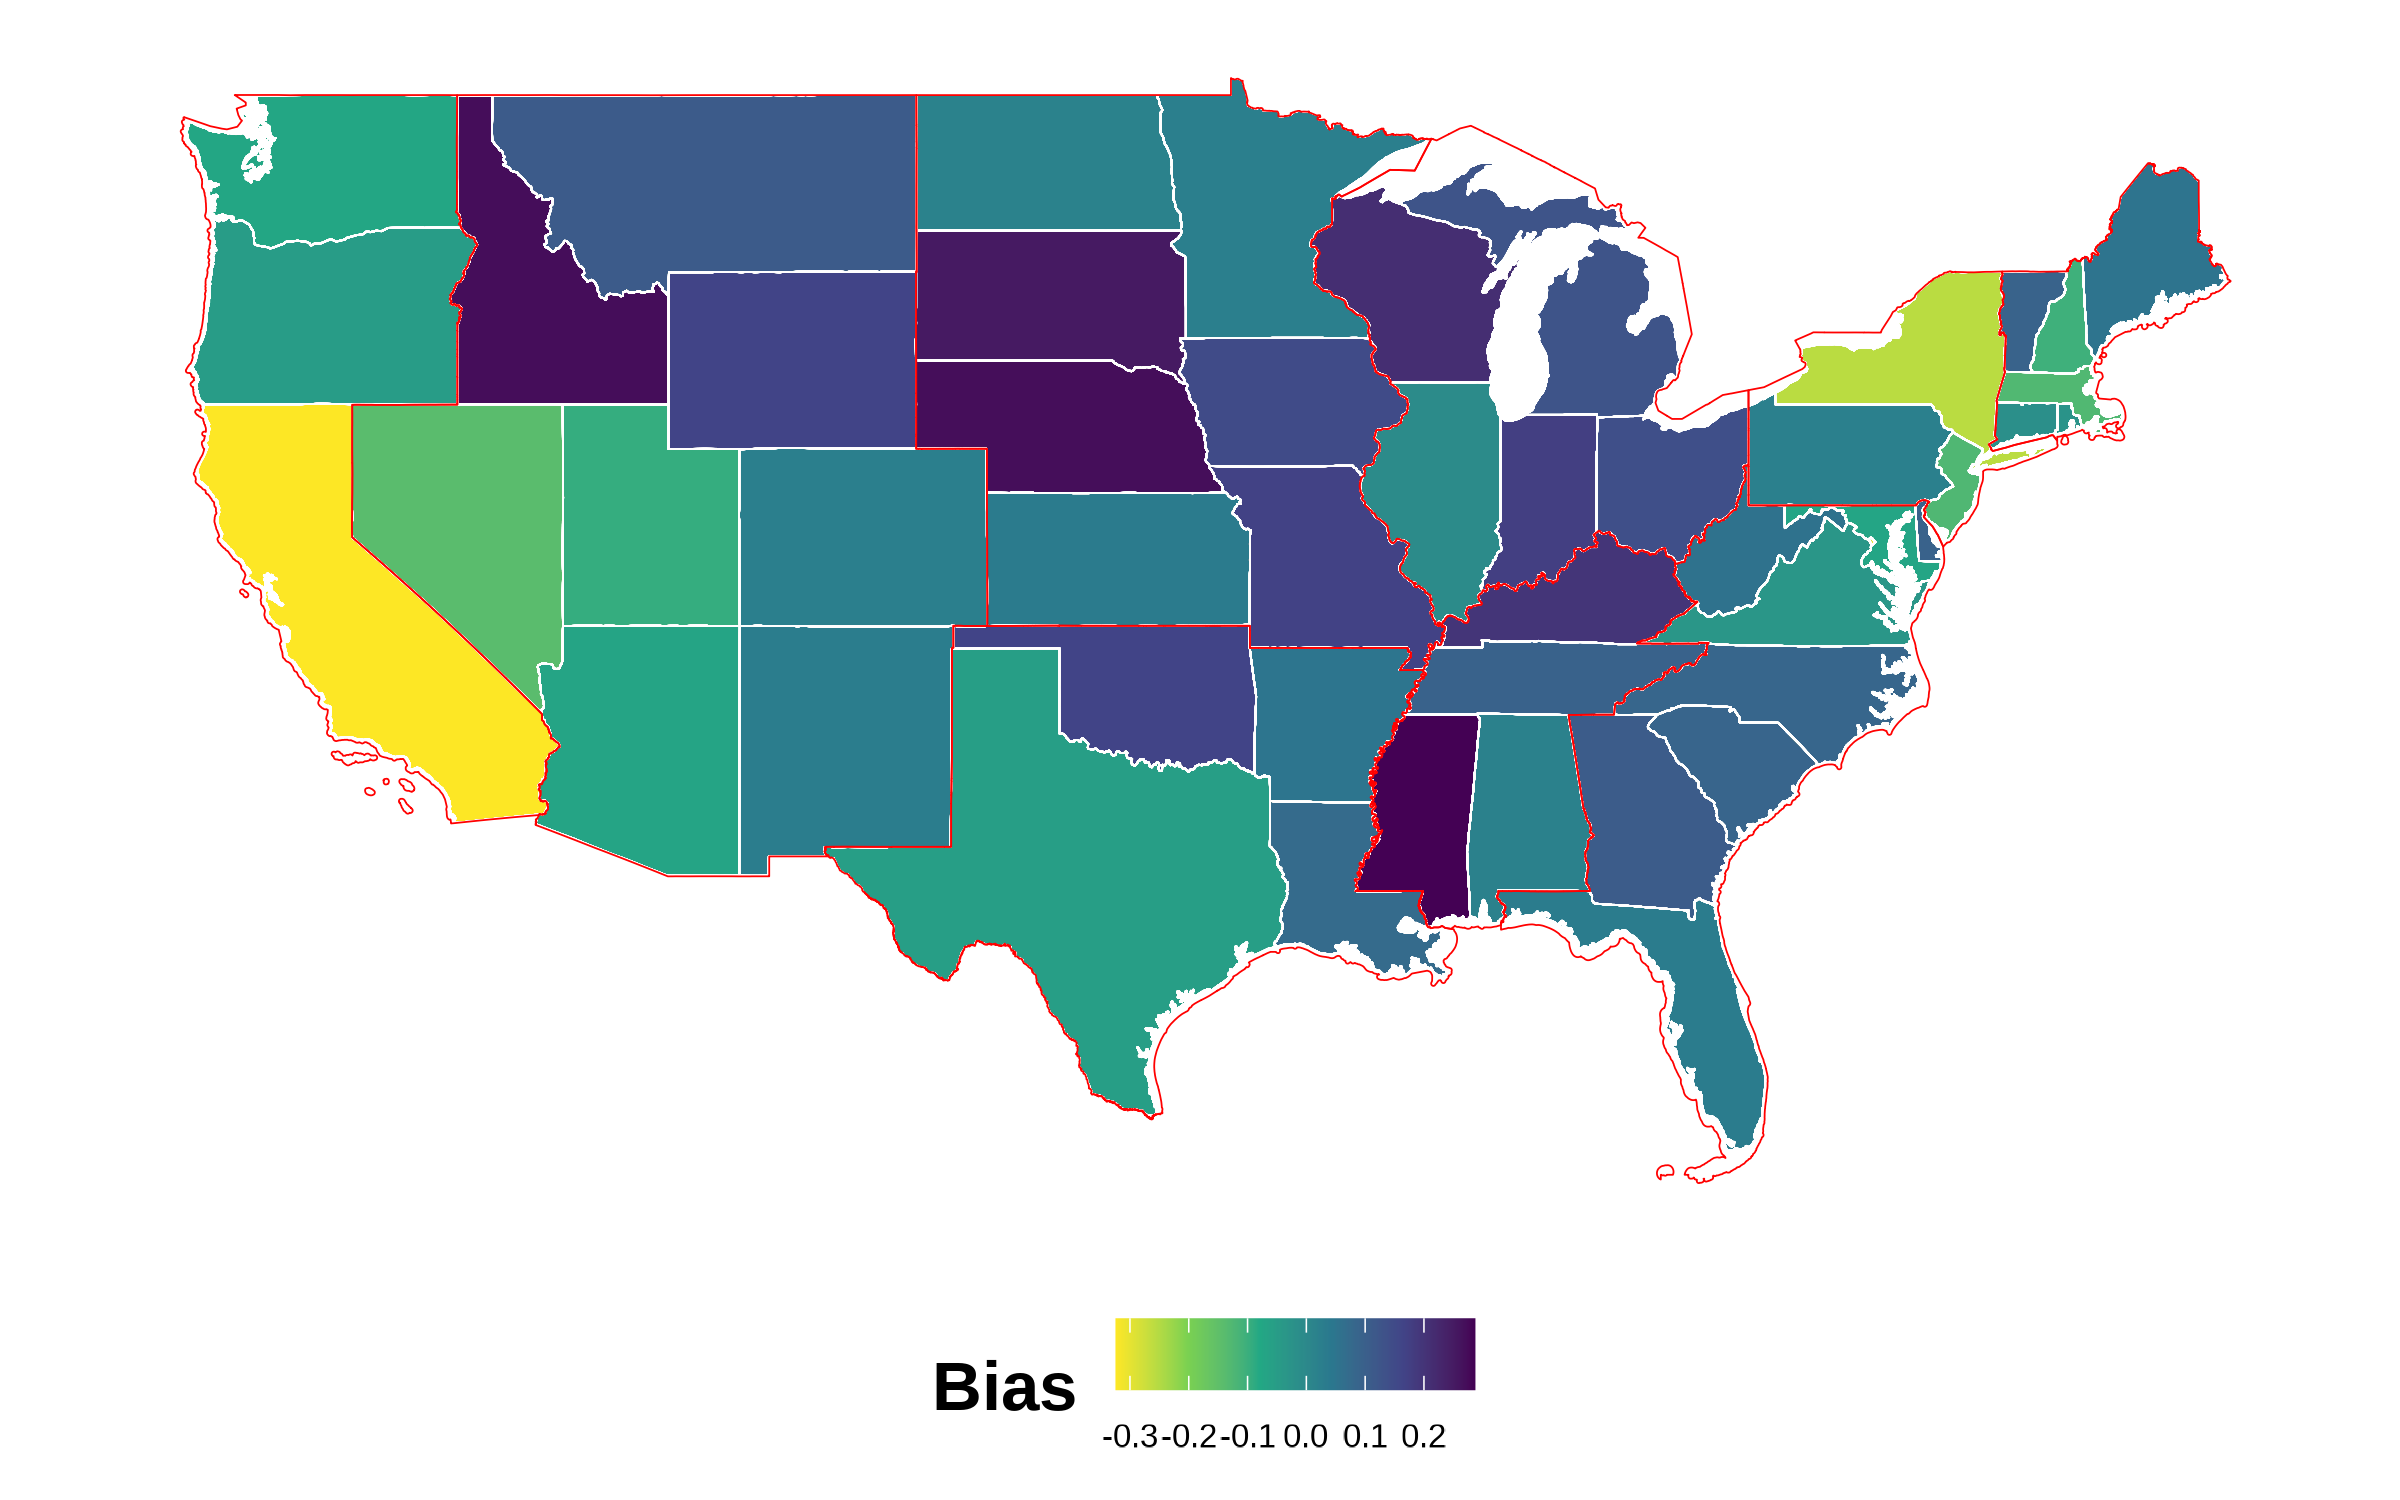
\includegraphics[width=0.9\linewidth]{figure/2018skinmap.png} 
\label{fig:skiniat-map-2018}
\hfill%
\end{subfigure}
\caption*{\footnotesize{In this figure, I show the state-level implicit bias in different years in the sample. Each panel presents state-level bias during a certain year. The boundaries in red represent the different Census divisions in the United States. Notice how there is a variation across states with-in a region.}}
\end{figure}
\end{center}

\begin{center}
\begin{figure}[!htb]
\centering
\caption{Relationship Between Self-Reported Asian Identity and Bias: By Generation}
\label{plot01-regression-gen}
%First graph
\begin{subfigure}{.48\textwidth}
\caption{All Generations}
\centering
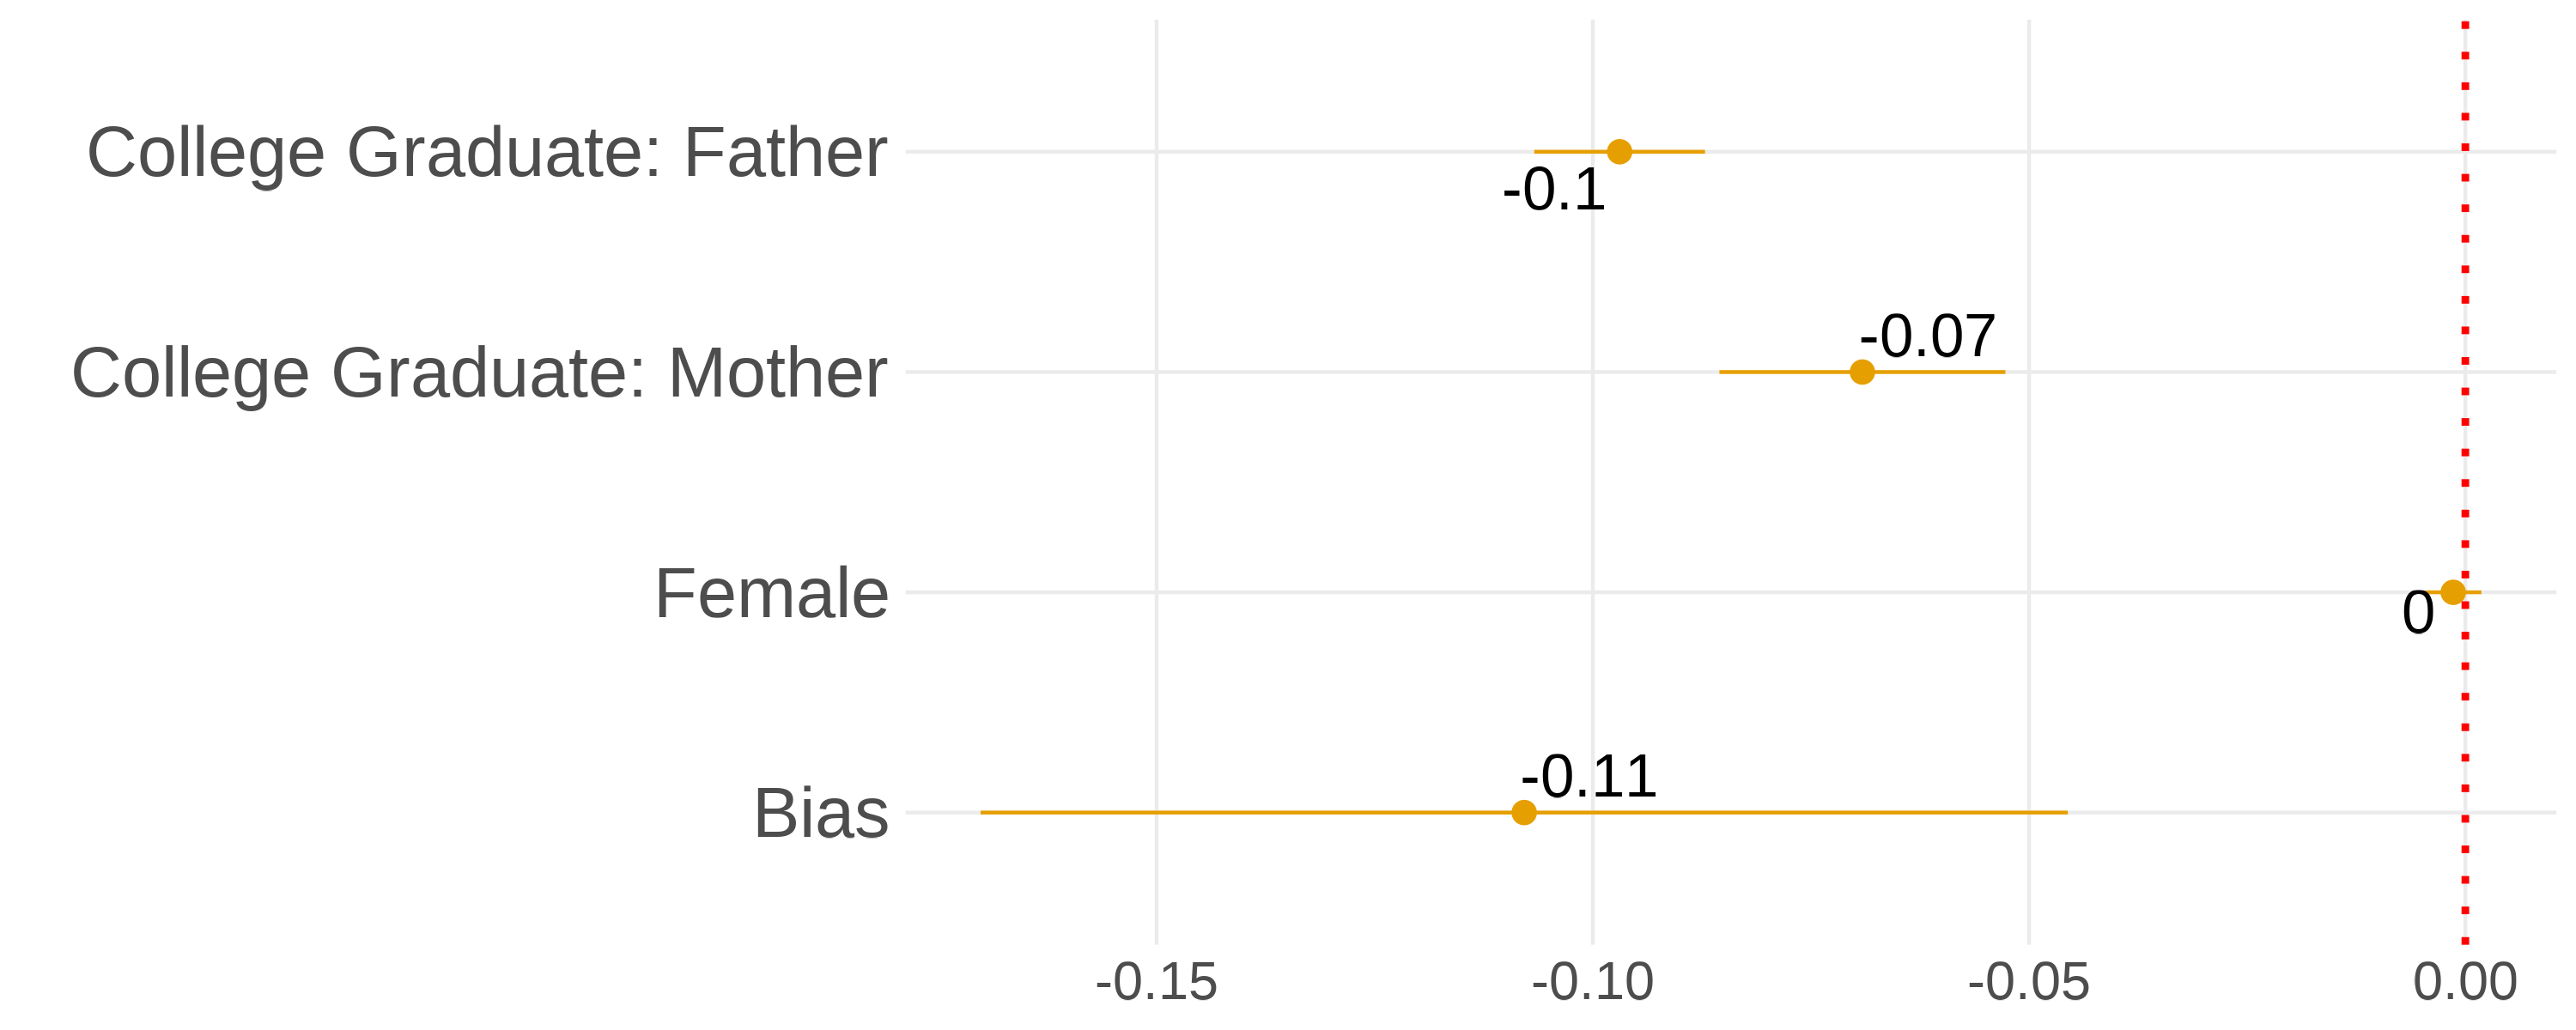
\includegraphics[width=.9\linewidth]{figure/skin-iat-regression-all-gens.png}
\end{subfigure}
\centering
%Second graph
\begin{subfigure}{.48\textwidth}
\caption{First-Generation}
\centering
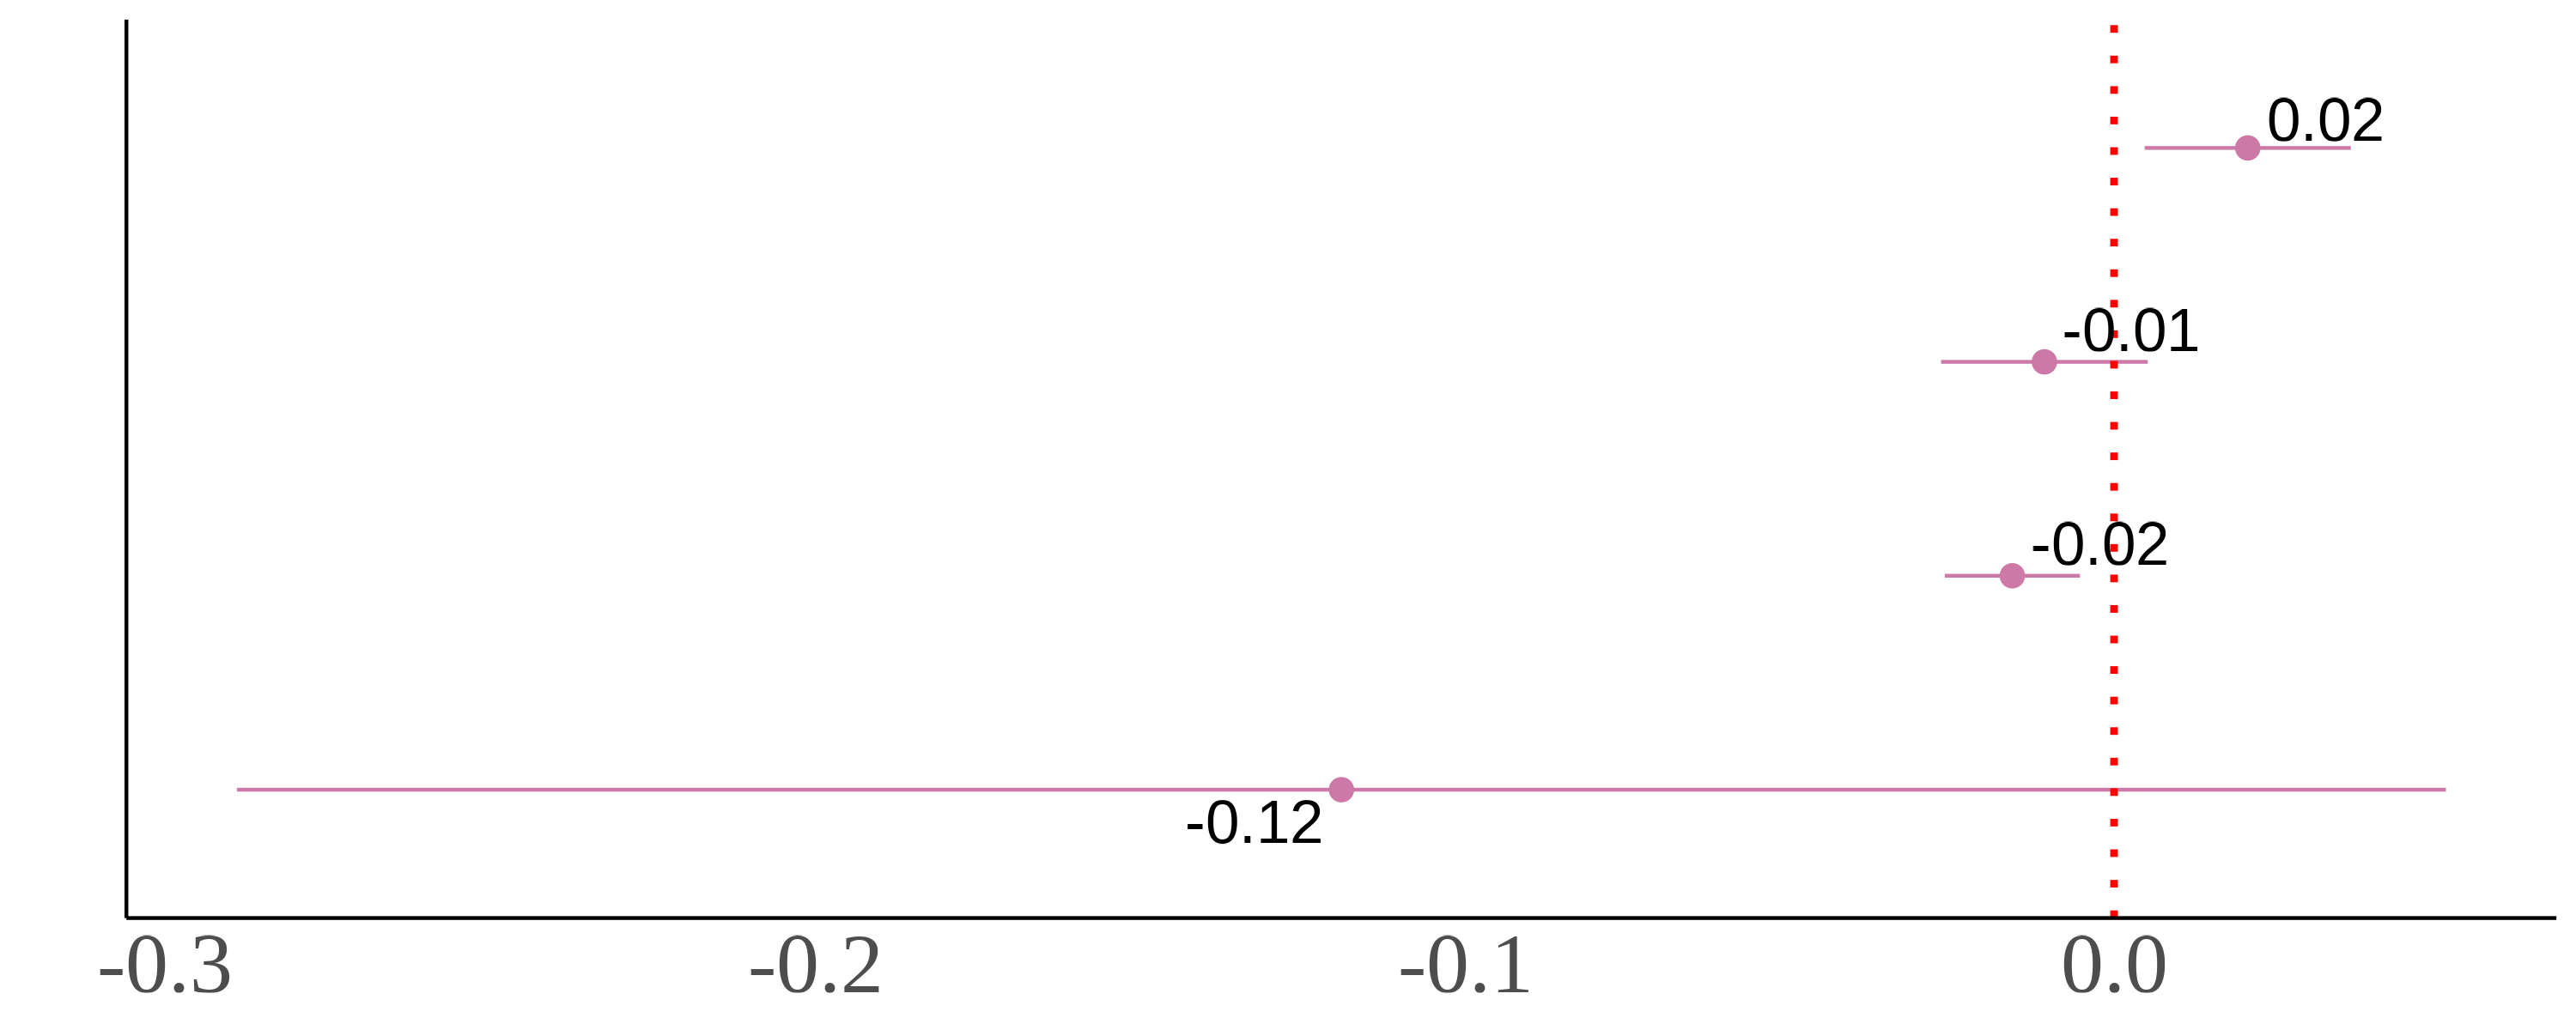
\includegraphics[width=.9\linewidth]{figure/skin-iat-regression-first-gen.png}
\end{subfigure}
%Third Graph
\begin{subfigure}{.48\textwidth}
\caption{Second-Generation}
\centering
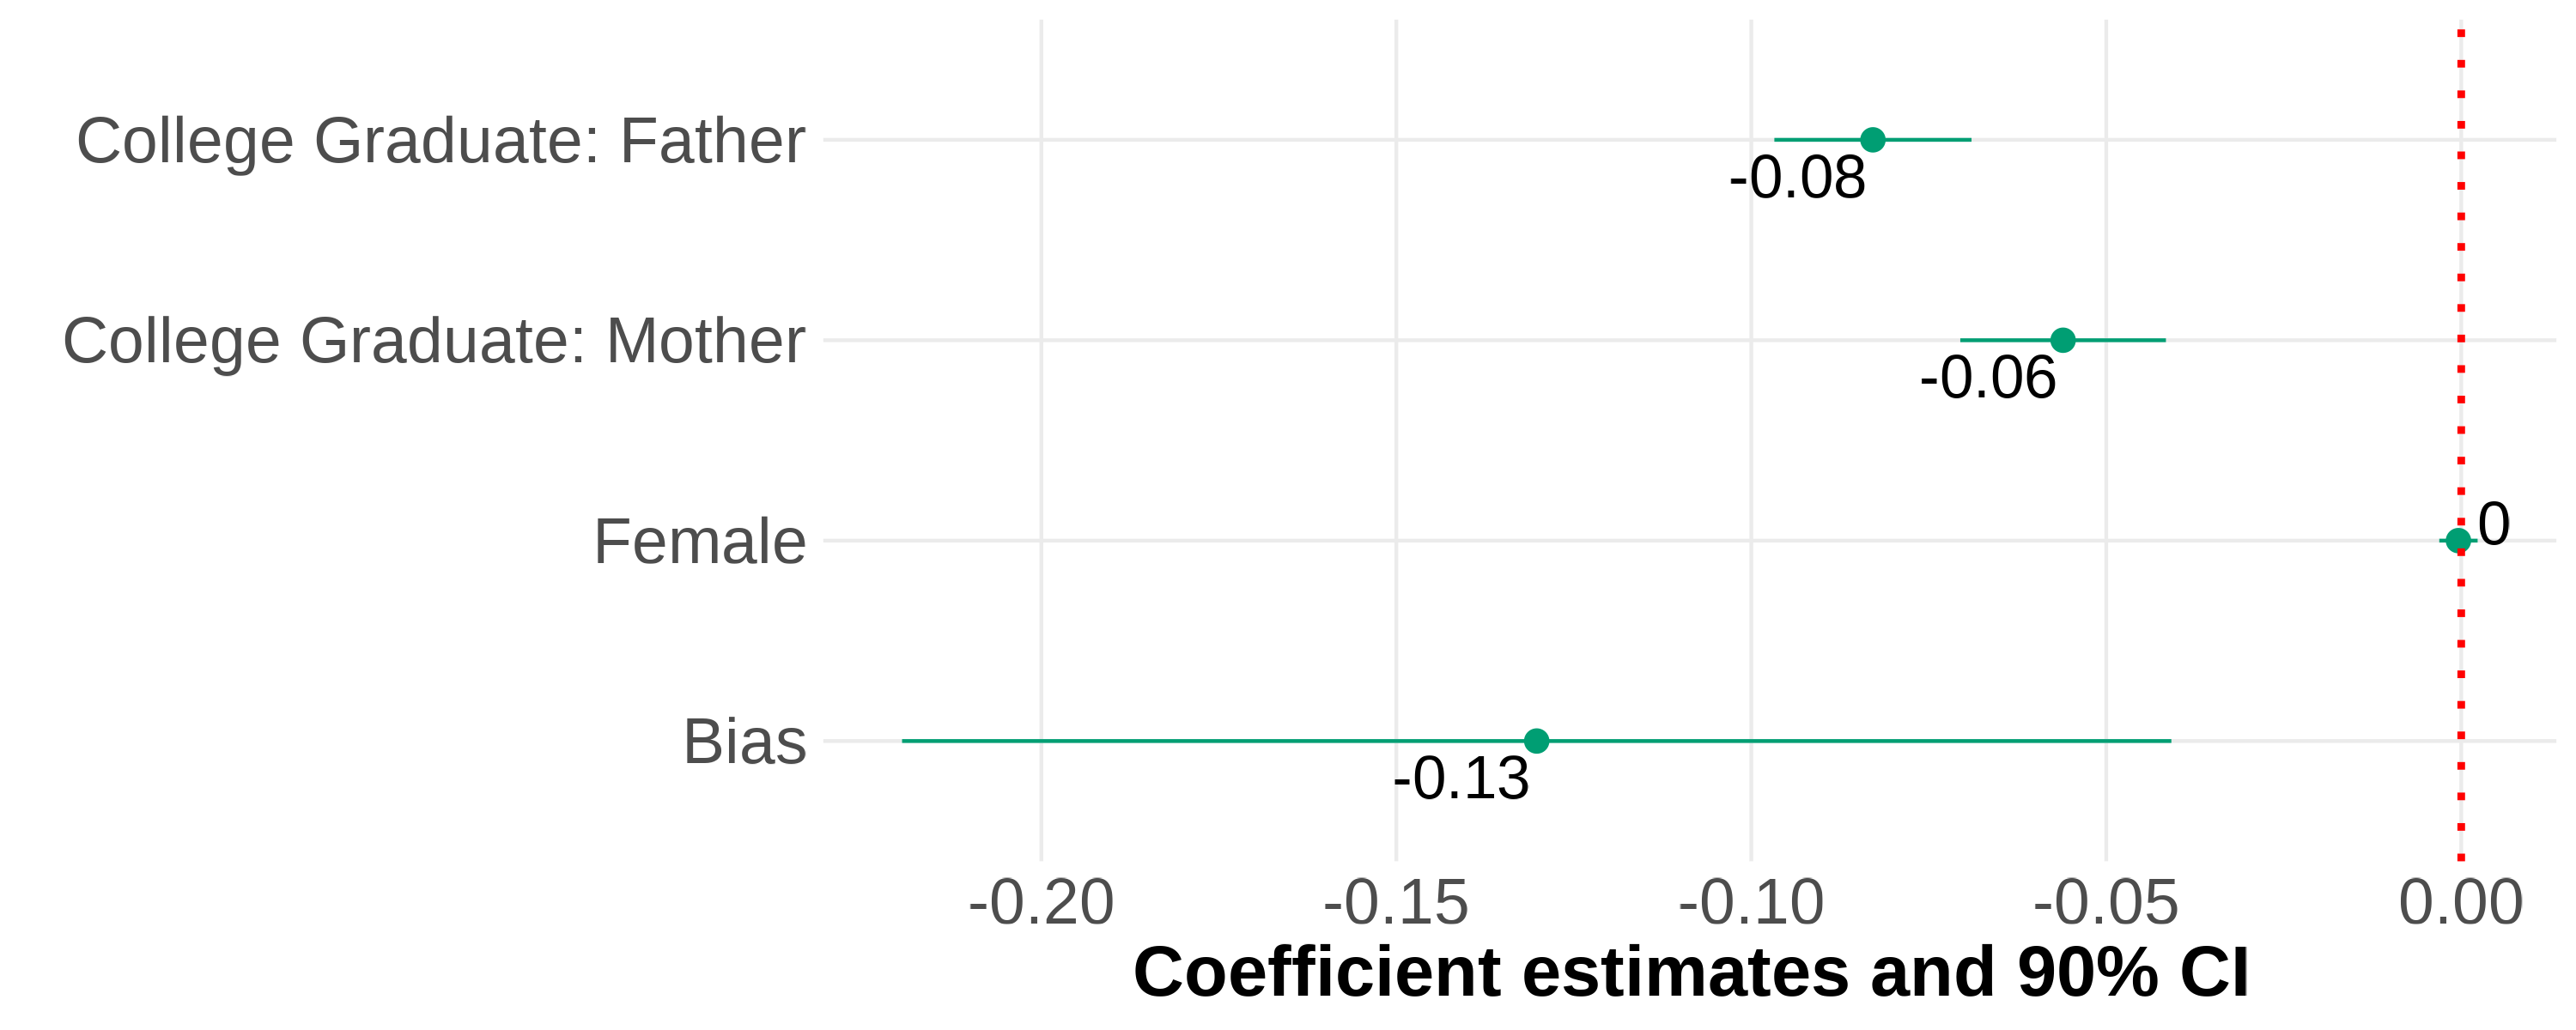
\includegraphics[width=.9\linewidth]{figure/skin-iat-regression-second-gen.png}
\end{subfigure}
%Fourth Graph
\begin{subfigure}{.48\textwidth}
\caption{Third-Generation}
\centering
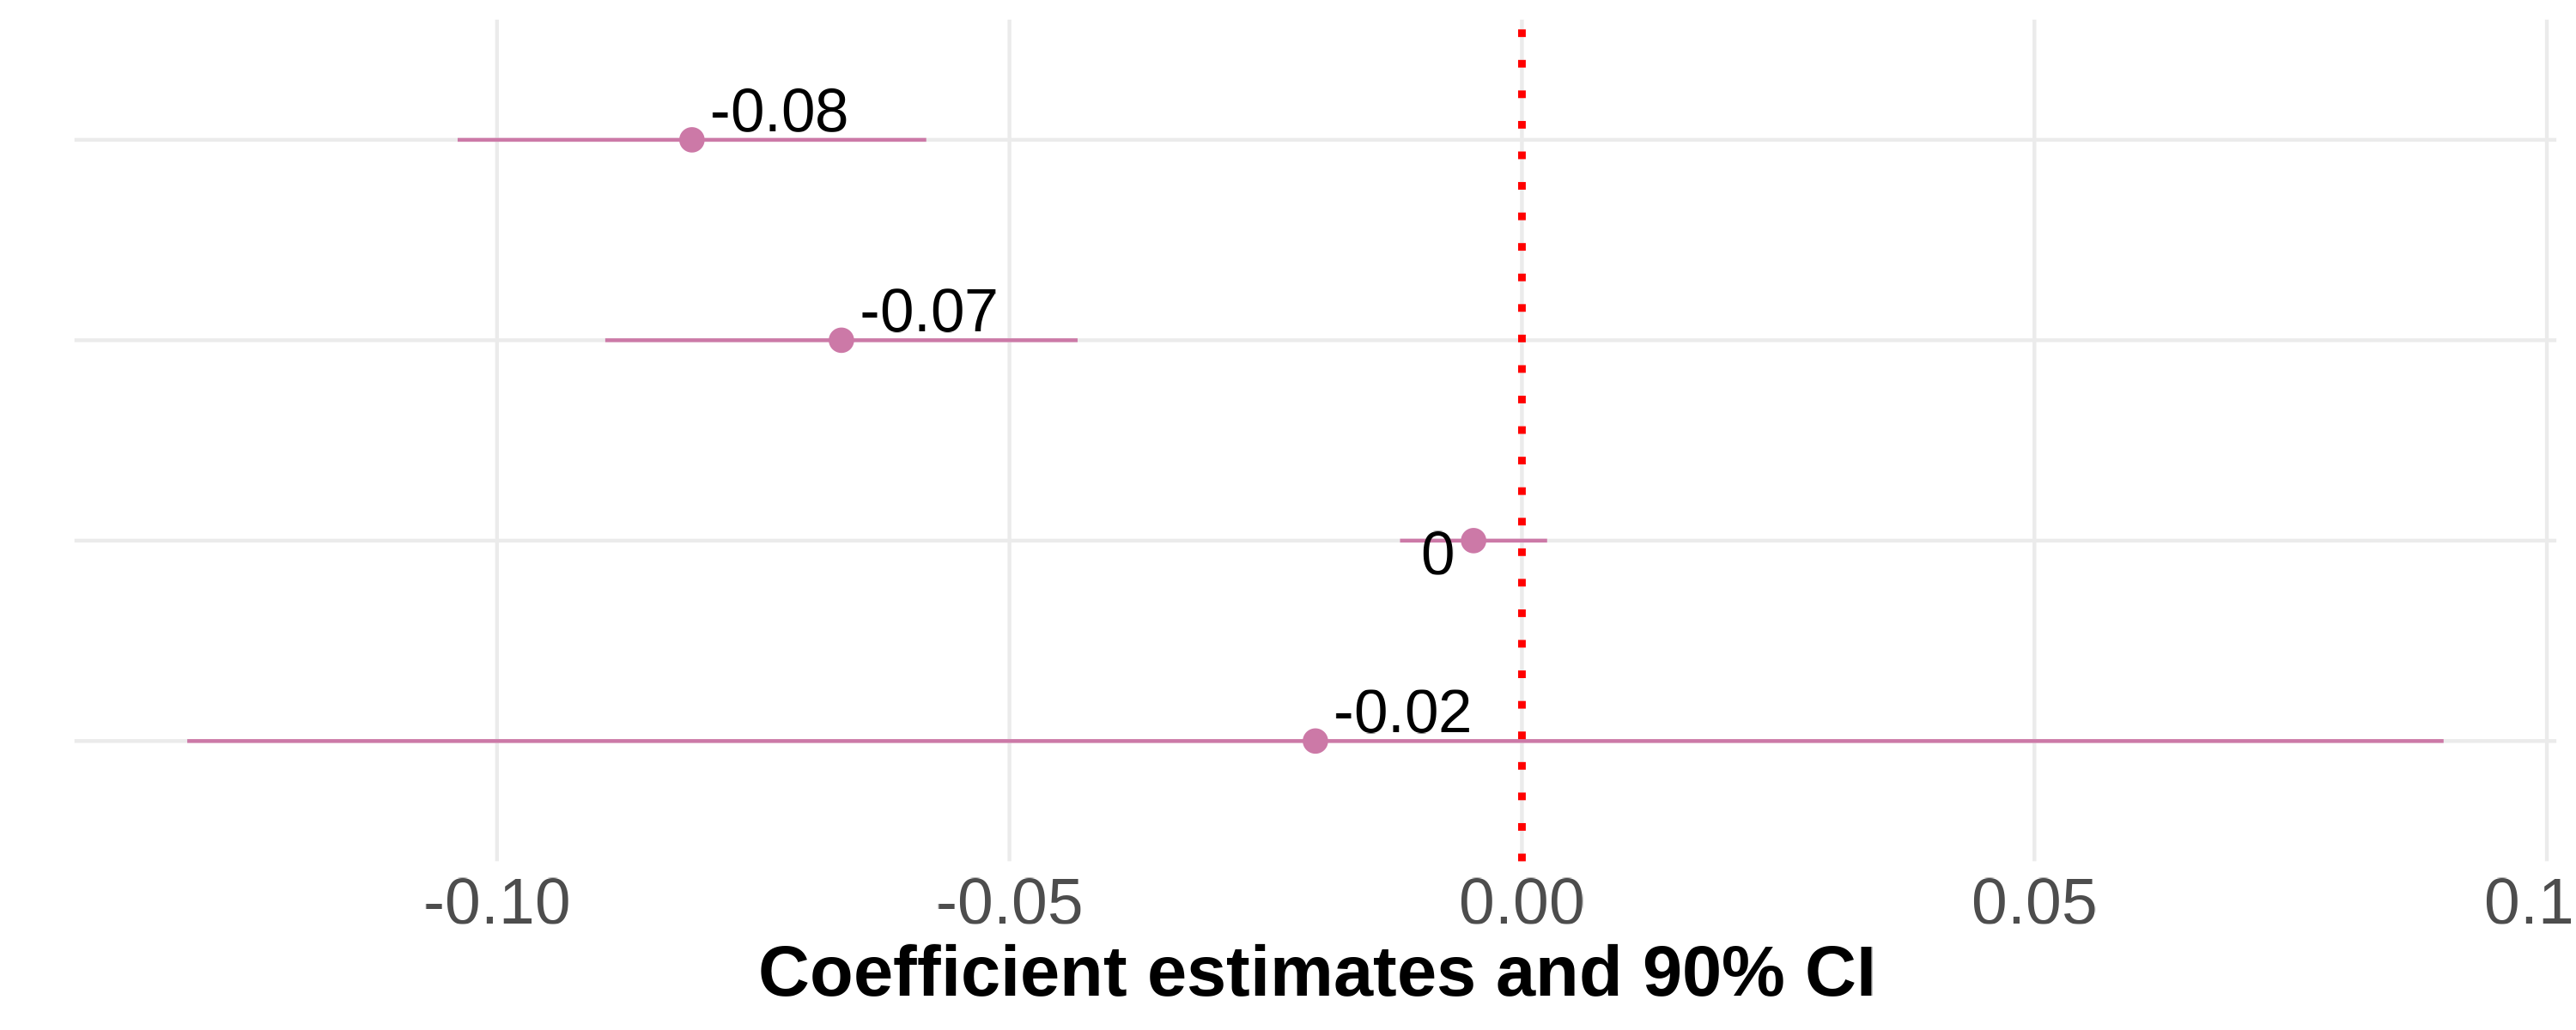
\includegraphics[width=.9\linewidth]{figure/skin-iat-regression-third-gen.png}
\end{subfigure}
\caption*{\footnotesize{I show four panels of estimating equation (\ref{eq:identity_reg_bias}). I include region $\times$ year fixed effects with controls for sex, quartic age, and parental education. The dependent variable is self-reported Asian identity and the independent variable is state-level bias. Each panel is the results from the same regression but on different samples that are divided by generation. Standard errors are clustered on the state level. The samples include first-, second-, and third-generation Asian children ages 17 and below who live in intact families. First-generation Asian immigrants are children that were born in a Asian country. Native-born second-generation Asian immigrants are children with at least one parent born in a Asian country. Finally, native-born third-generation Asian immigrants are children with native-born parents and at least one grandparent born in a Asian country.}}
\end{figure}
\end{center}

\pagebreak
\newpage

\begin{center}
\begin{figure}[!htb]
\centering
\caption{Relationship Between Self-Reported Hispanic Identity and Bias: By Parental Types}
\label{plot01-regression-byparent}
%First graph
\begin{subfigure}{.48\textwidth}
\caption{Second-Generation (All Parental Types)}
\centering
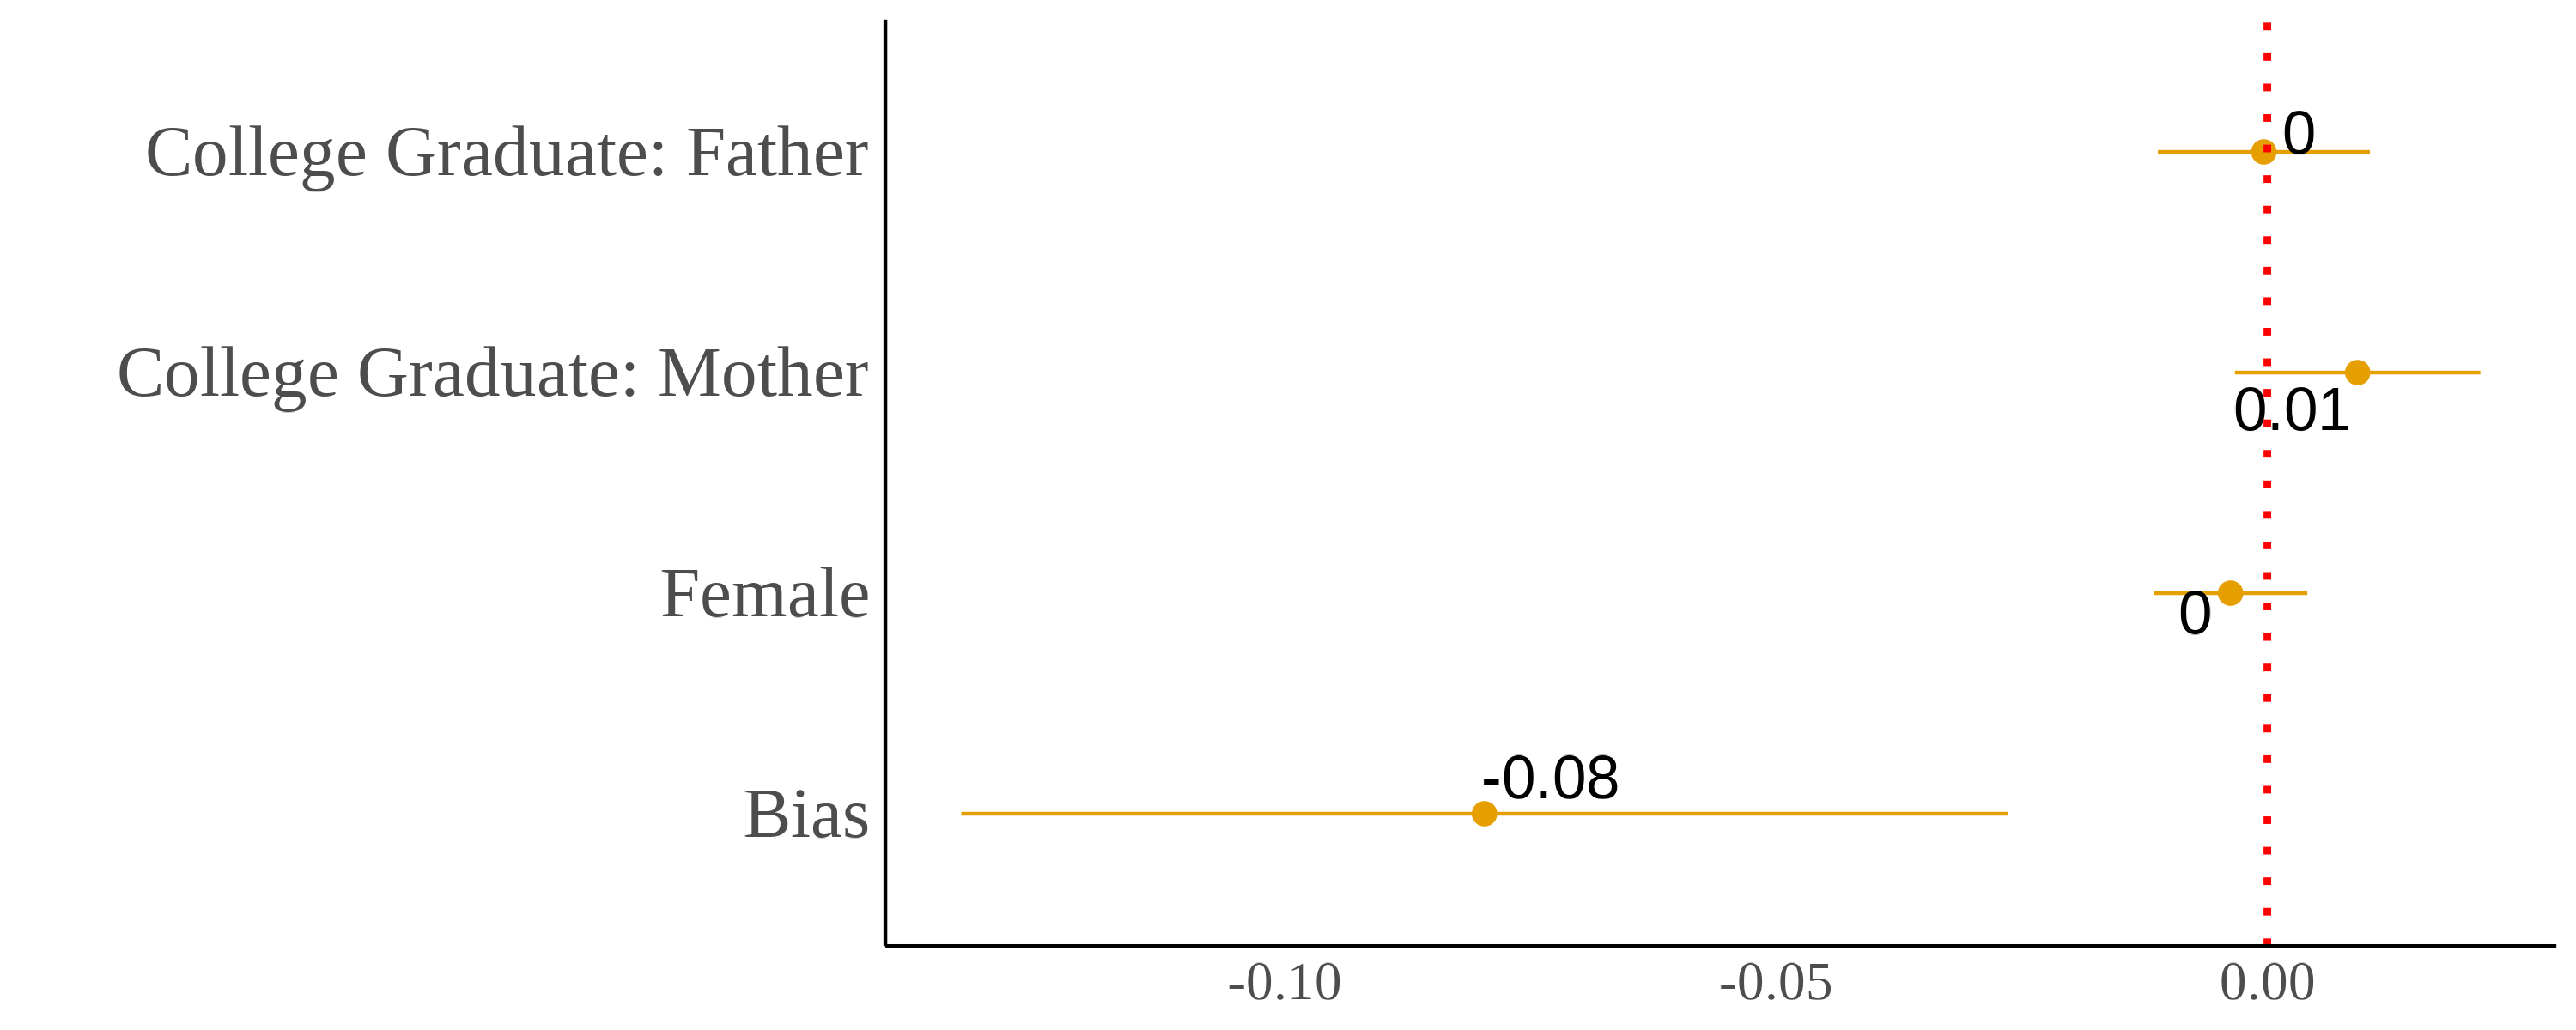
\includegraphics[width=.9\linewidth]{figure/by-parents-regs-all.png}
\end{subfigure}
\centering
%Second graph
\begin{subfigure}{.48\textwidth}
\caption{Hispanic Fathers-Hispanic Mothers}
\centering
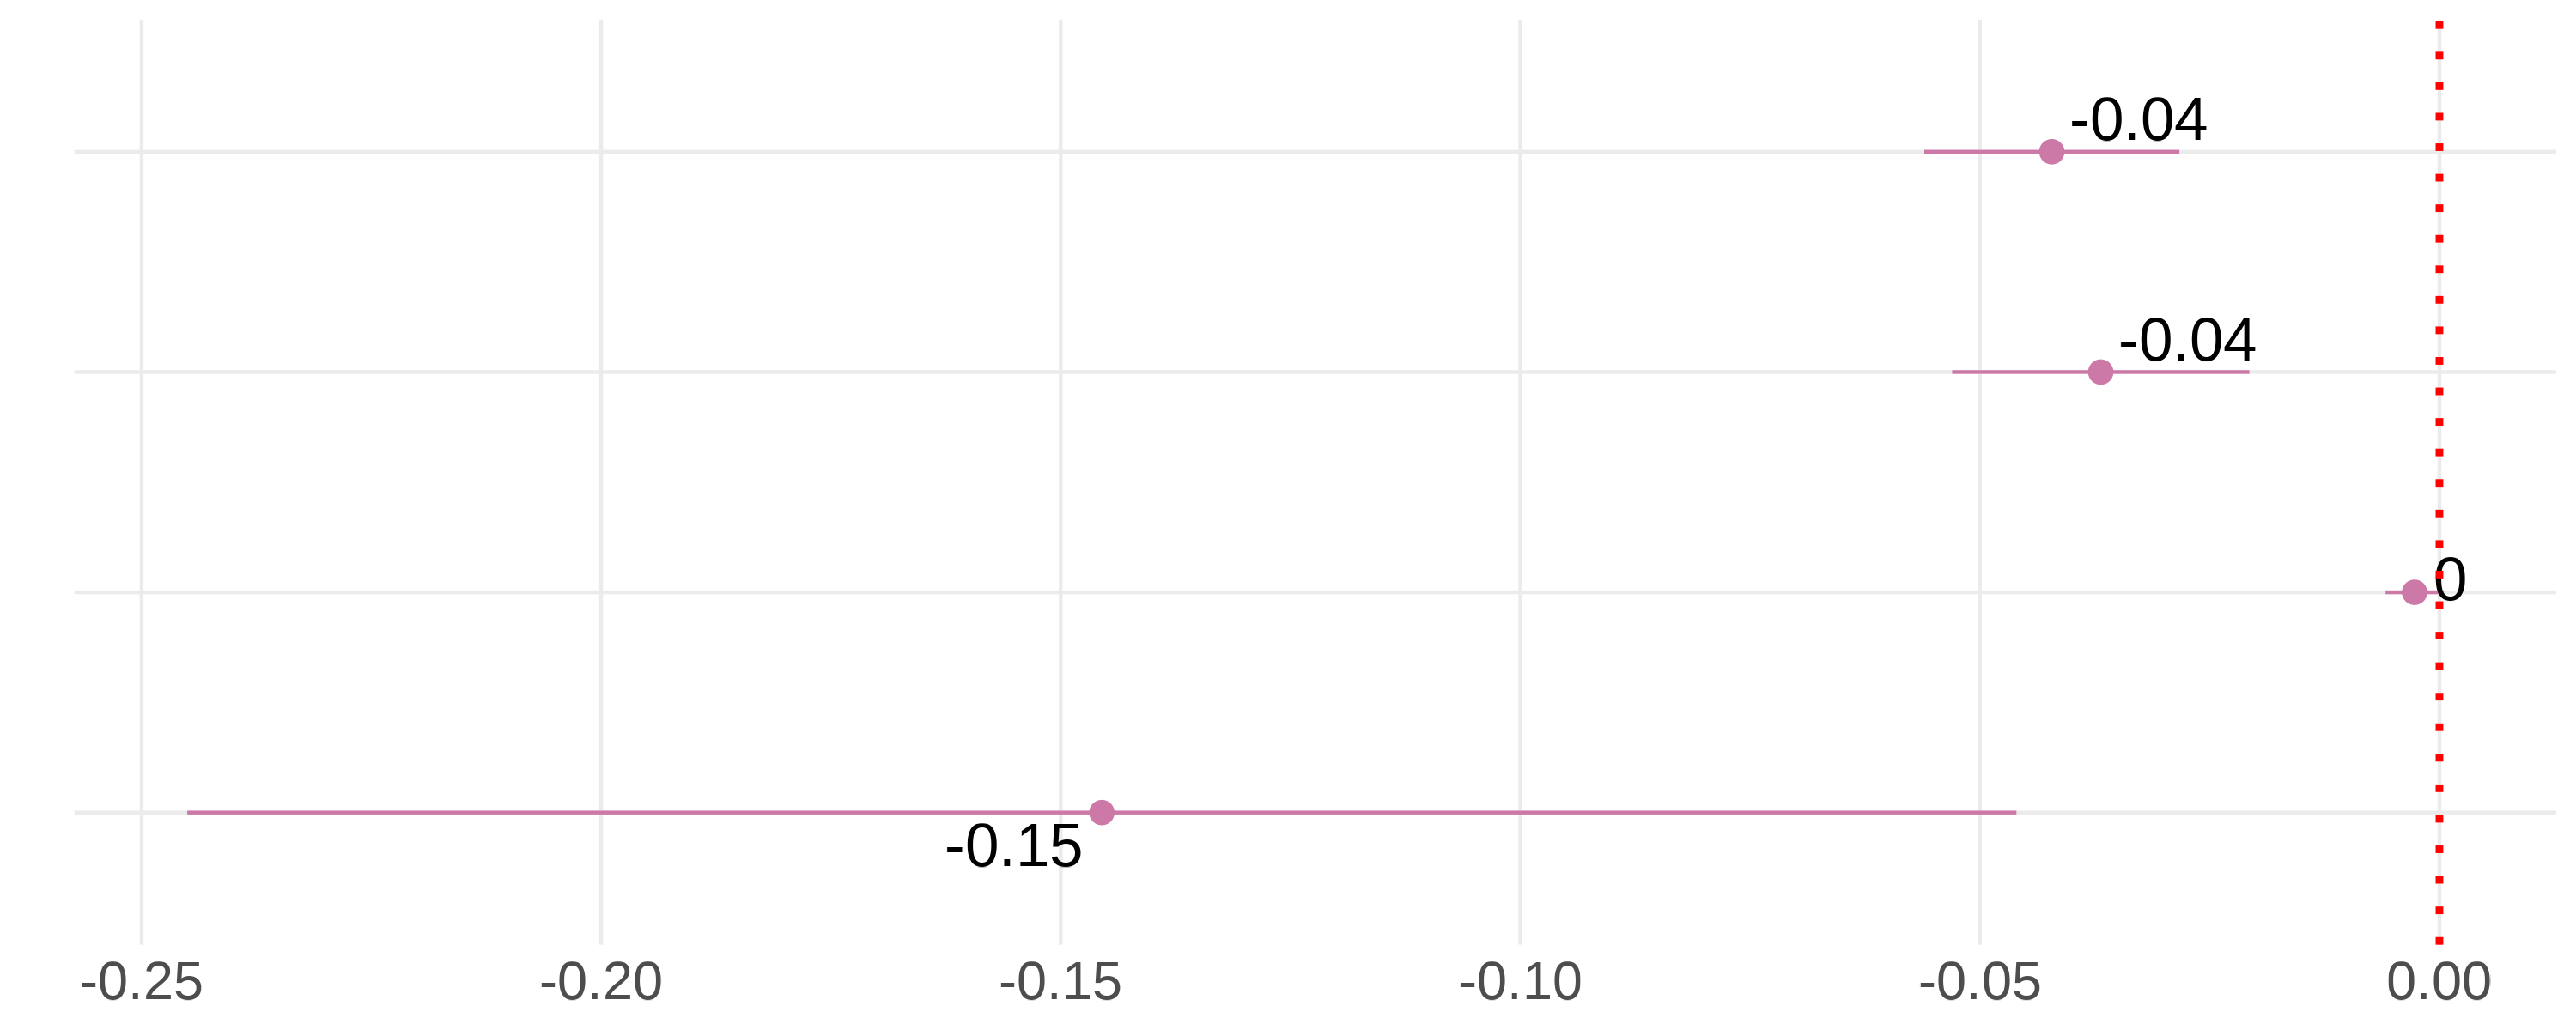
\includegraphics[width=.9\linewidth]{figure/by-parents-regs-hh.png}
\end{subfigure}
%Third Graph
\begin{subfigure}{.48\textwidth}
\caption{Hispanic Fathers-White Mothers}
\centering
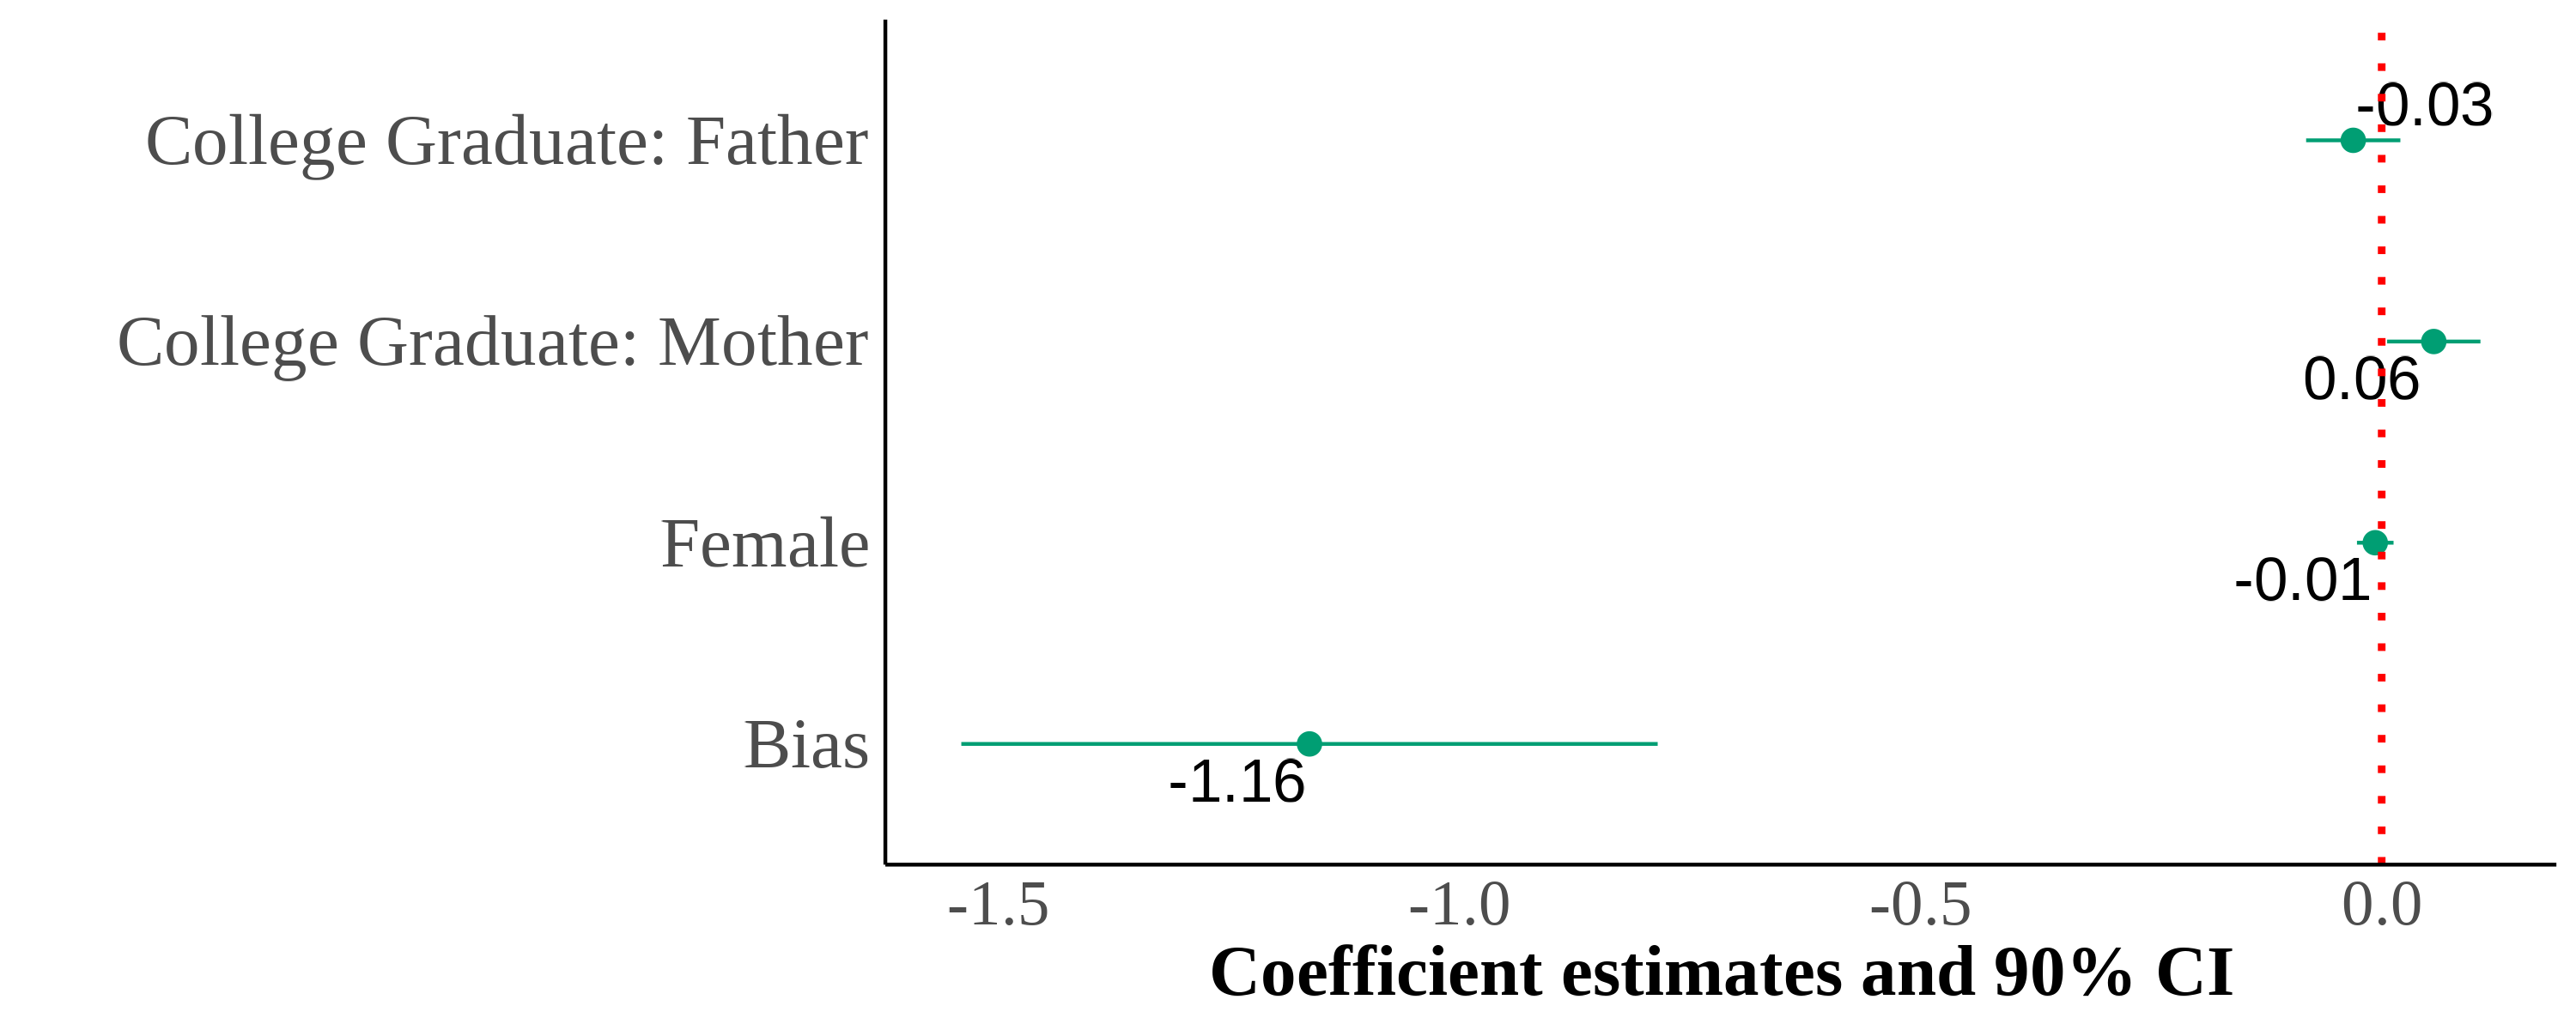
\includegraphics[width=.9\linewidth]{figure/by-parents-regs-hw.png}
\end{subfigure}
%Fourth Graph
\begin{subfigure}{.48\textwidth}
\caption{White Fathers-Hispanic Mothers}
\centering
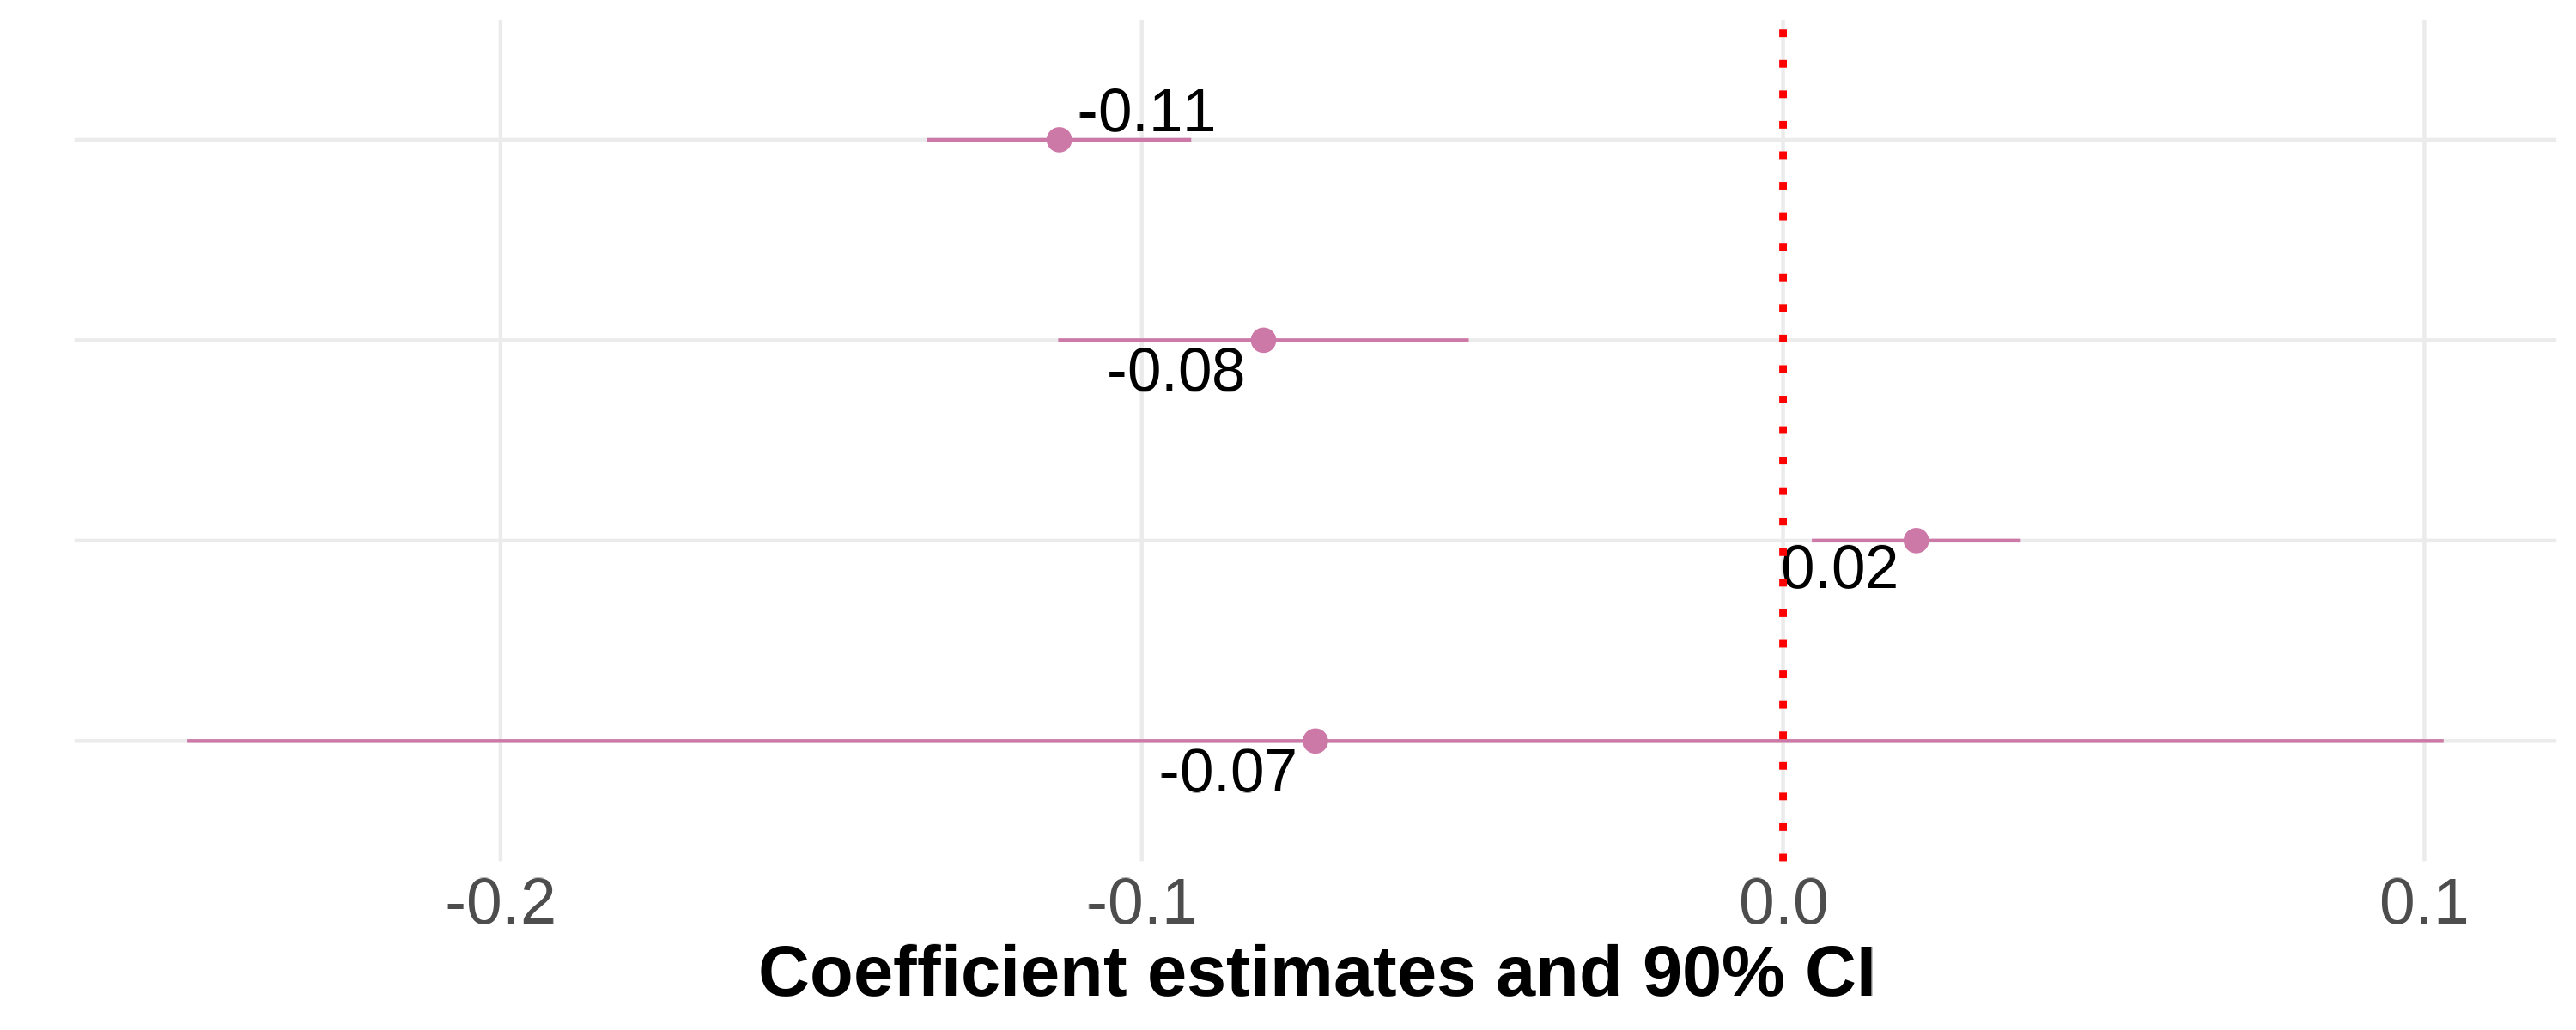
\includegraphics[width=.9\linewidth]{figure/by-parents-regs-wh.png}
\end{subfigure}
\caption*{\footnotesize{I show four panels of estimating equation (\ref{eq:identity_reg_bias}). I include region $\times$ year fixed effects with controls for sex, quartic age, and parental education. The dependent variable is self-reported Hispanic identity and the independent variable is state-level bias. Each panel results from the same regression but on different samples divided by parental types. Standard errors are clustered on the state level. The samples include second-generation Hispanic children ages 17 and below who live in intact families. Native-born second-generation Hispanic immigrant children with at least one parent born in a Spanish-speaking country.}}
\end{figure}
\end{center}

\pagebreak
\newpage

\begin{table}[H]

\caption{Relationship Between Bias and Self-Reported Hispanic identity Among Third-Generation Hispanic Immigrants: By Grandparental Type \label{regtab-bygrandparents}}
\centering
\resizebox{\linewidth}{!}{
\begin{threeparttable}
\begin{tabular}[t]{lcccc}
\toprule
\multicolumn{1}{c}{ } & \multicolumn{4}{c}{Number of Hispanic Grandparents} \\
\cmidrule(l{3pt}r{3pt}){2-5}
  & \specialcell{(1) \\ One} & \specialcell{(2) \\ Two} & \specialcell{(3) \\ Three} & \specialcell{(4) \\ Four}\\
\midrule
Bias & -0.04 & 0.03 & 0.19 & -0.14*\\
 & (0.11) & (0.09) & (0.26) & (0.07)\\
Female & -0.01 & 0.00 & -0.01 & 0.00\\
 & (0.01) & (0.01) & (0.01) & (0.01)\\
College Graduate: Mother & -0.11*** & -0.07*** & 0.02 & -0.02\\
 & (0.03) & (0.02) & (0.02) & (0.01)\\
College Graduate: Father & -0.11*** & -0.08*** & 0.02 & -0.03*\\
 & (0.03) & (0.01) & (0.01) & (0.01)\\
\midrule
Observations & 55,051 & 74,100 & 12,194 & 57,646\\
Year $\times$ Region FE & X & X & X & X\\
\bottomrule
\multicolumn{5}{l}{\rule{0pt}{1em}* p $<$ 0.1, ** p $<$ 0.05, *** p $<$ 0.01}\\
\end{tabular}
\begin{tablenotes}
\small
\item[1] \footnotesize{Each column is an estimation of equation (\ref{eq:identity_reg_bias}) restricted to third-generation Hispanic immigrants by 
                      number of Hispanic grandparents with region × year fixed effects. 
                      I include controls for sex, quartic age, fraction of Hispanics in a state, and parental education.
                      Standard errors are clustered on the state level.}
\item[2] \footnotesize{The samples include third-generation Hispanic children ages 17 and below who live in intact families. 
                      Native-born third-generation Hispanic 
                      immigrant children with at least one grandparent born in a Spanish-speaking 
                      country.}
\item[3] \footnotesize{Data source is the 2004-2021 Current Population Survey.}
\end{tablenotes}
\end{threeparttable}}
\end{table}


\begin{table}[H]
\centering\centering
\caption{Relationship Between Bias and Interethnic Marriages \label{regtab-logit-02}}
\centering
\begin{threeparttable}
\begin{tabular}[t]{lccc}
\toprule
\multicolumn{2}{c}{ } & \multicolumn{1}{c}{Asian Men} & \multicolumn{1}{c}{Asian Women} \\
\cmidrule(l{3pt}r{3pt}){3-3} \cmidrule(l{3pt}r{3pt}){4-4}
  & \specialcell{(1) \\ Interethnic} & \specialcell{(2) \\ Interethnic} & \specialcell{(3) \\ Interethnic}\\
\midrule
Bias & $0.04$*** & $-0.01$ & $0.03$**\\
 & ($0.01$) & ($0.01$) & ($0.01$)\\
College Graduate: Wife & $0.04$*** & $0.04$*** & $0.05$***\\
 & ($0.00$) & ($0.01$) & \vphantom{1} ($0.00$)\\
College Graduate: Husband & $-0.01$* & $-0.01$ & $-0.02$***\\
 & ($0.00$) & ($0.01$) & ($0.00$)\\
\midrule
Observations & $69,800$ & $52,103$ & $60,214$\\
Year $\times$ Region FE & X & X & X\\
\bottomrule
\multicolumn{4}{l}{\rule{0pt}{1em}* p $<$ 0.1, ** p $<$ 0.05, *** p $<$ 0.01}\\
\end{tabular}
\begin{tablenotes}
\small
\item[1] \footnotesize{This is the result to estimating (\ref{eq:inter-interethnic}) as a
                      linear probability model.}
\item[2] \footnotesize{I include controls for partners' sex, age, education, 
                      and years since immigrating to the United States.
                      Standard errors are clustered on the household level.}
\item[3] \footnotesize{Data source is the 2004-2020 Current Population Survey Data.}
\end{tablenotes}
\end{threeparttable}
\end{table}


\begin{table}[H]
\centering\centering
\caption{Main Effect of Proxy on Second-Generation's Asian Self-identification \label{tab:hispbyproxy}}
\centering
\fontsize{12}{14}\selectfont
\begin{tabular}[c]{>{}lllll}
\toprule
Parents Type & All & Asian-Asian & Asian-White & White-Asian\\
\midrule
\textbf{Proxy:} &  &  &  & \\
\hspace{1em}\textbf{Mother} & 0.72 & 0.97 & 0.37 & 0.3\\
\hspace{1em}\textbf{Father} & 0.72 & 0.97 & 0.39 & 0.29\\
\hspace{1em}\textbf{Self} & 0.87 & 0.97 & 0.23 & 0.31\\
\hspace{1em}\textbf{Others} & 0.88 & 0.96 & 0.6 & 0.54\\
\bottomrule
\end{tabular}
\end{table}


\begin{table}[H]
\centering\centering
\caption{Relationship Between Bias and Migration \label{regtab-mig-01}}
\centering
\resizebox{0.7\textwidth}{!}{
\begin{threeparttable}
\begin{tabular}[t]{lccc}
\toprule
  & \specialcell{(1) \\ Migrated from \\ Birth Place} & \specialcell{(2) \\ Migrated from \\ Birth Place} & \specialcell{(3) \\ $Bias_{ist} - Bias_{ilb}$}\\
\midrule
$Bias_{st}$ & 0.13* &  & \\
 & (0.07) &  & \\
$Bias_{lb}$ &  & -0.03 & \\
 &  & (0.17) & \\
Asian &  &  & 0.02\\
 &  &  & (0.04)\\
Female & 0.00 & -0.01 & 0.00\\
 & (0.00) & (0.00) & (0.02)\\
College Graduate: Mother & 0.01*** & 0.00 & -0.01\\
 & (0.00) & (0.01) & (0.03)\\
College Graduate: Father & -0.03*** & -0.03*** & 0.03\\
 & (0.01) & (0.01) & (0.02)\\
\midrule
Observations & 73,563 & 41,641 & 2,075\\
Mean & 0.15 & 0.15 & -0.1\\
Year $\times$ Region FE & X &  & \\
Birthyear $\times$ Birth Region FE &  & X & \\
\bottomrule
\multicolumn{4}{l}{\rule{0pt}{1em}* p $<$ 0.1, ** p $<$ 0.05, *** p $<$ 0.01}\\
\end{tabular}
\begin{tablenotes}
\small
\item[1] \footnotesize{Each column is an estimation of equations (\ref{eq:migration-3}) in column (1), 
                      (\ref{eq:migration-4}) in column (2), and
                      (\ref{eq:migration-5}) in column (3).}
\item[2] \footnotesize{Column (1) is a regression where the left hand side variable is 
                      a dummy variable that is equal to one if a person migrated from the state
                      were born in and the right hand side variable is bias the year of survey.
                      Column (2) is a regression where the left hand side variable is 
                      a dummy variable that is equal to one if a person migrated from the state
                      were born in and the right hand side variable is bias the year of birth in the state of birth.
                      Column (3) is a regression where the left hand side variable is 
                      the difference between state-level bias during the year of the survey in the current state the 
                      respondent is living in, and state-level bias during the year of birth in the state of birth 
                      and the right hand side variable is self-reported Asian identity. This regression captures
                      the selection of those that self-reported Asian identity into states with different levels of bias.
                      I include controls for sex, quartic age, parental education, fraction of Asians in a state, and region × year fixed effects.
                      Standard errors are clustered on the state level.}
\item[3] \footnotesize{The samples include children ages 17 and below who live in intact families. 
                      Native-born second-generation Asian immigrant children with both
                      parents born in a Asian country. The sample in the column (3) regression is further restricted to only those that migrated from their birth state.}
\item[4] \footnotesize{Data source is the 2004-2021 Census Data.}
\end{tablenotes}
\end{threeparttable}}
\end{table}


\pagebreak
\begingroup
\setstretch{1.0}
%\setstretch{1.1}
\setlength\bibitemsep{0pt}
\printbibliography
\endgroup
\pagebreak

\begin{appendices}

\section{Tables}\label{appendix:tabs}

% \begin{table}[!h]
\centering\centering
\caption{Relationship Between Bias and Self-Reported Asian Identity: By Proxy Respondent\label{regtab-proxy-01}}
\centering
\resizebox{\ifdim\width>\linewidth\linewidth\else\width\fi}{!}{
\begin{threeparttable}
\begin{tabular}[t]{lcccccc}
\toprule
\multicolumn{1}{c}{ } & \multicolumn{6}{c}{Proxy Respondent} \\
\cmidrule(l{3pt}r{3pt}){2-7}
\multicolumn{1}{c}{ } & \multicolumn{1}{c}{White Mother} & \multicolumn{1}{c}{Asian Mother} & \multicolumn{1}{c}{White Father} & \multicolumn{1}{c}{Asian Father} & \multicolumn{1}{c}{Self} & \multicolumn{1}{c}{Other} \\
\cmidrule(l{3pt}r{3pt}){2-2} \cmidrule(l{3pt}r{3pt}){3-3} \cmidrule(l{3pt}r{3pt}){4-4} \cmidrule(l{3pt}r{3pt}){5-5} \cmidrule(l{3pt}r{3pt}){6-6} \cmidrule(l{3pt}r{3pt}){7-7}
  & \specialcell{(1) \\ $A_{ist}$} & \specialcell{(2) \\ $A_{ist}$} & \specialcell{(3) \\ $A_{ist}$} & \specialcell{(4) \\ $A_{ist}$} & \specialcell{(5) \\ $A_{ist}$} & \specialcell{(6) \\ $A_{ist}$}\\
\midrule
Prejudice Measure & 0.04 & -0.06 & -0.09 & 0.03 & 0.02 & 0.07\\
 & (0.07) & (0.05) & (0.06) & (0.03) & (0.07) & (0.06)\\
Female & -0.02 & 0.01 & -0.01 & 0.00 & -0.07* & 0.00\\
 & (0.02) & (0.01) & (0.02) & (0.01) & (0.04) & (0.01)\\
College Graduate: Mother & 0.01 & -0.04** & -0.02 & 0.00 & -0.05 & -0.07***\\
 & (0.03) & (0.01) & (0.02) & (0.01) & (0.05) & (0.01)\\
College Graduate: Father & 0.00 & 0.00 & 0.02 & 0.01 & -0.02 & -0.02\\
 & (0.03) & (0.02) & (0.02) & (0.01) & (0.06) & (0.01)\\
Second Gen & -0.06 & -0.10*** & 0.17 & -0.18*** & -1.02*** & -0.44***\\
 & (0.04) & (0.04) & (0.18) & (0.05) & (0.05) & (0.05)\\
\midrule
Observations & 4,330 & 28,374 & 8,686 & 28,506 & 738 & 5,823\\
Year $\times$ Region FE & X & X & X & X & X & X\\
\bottomrule
\multicolumn{7}{l}{\rule{0pt}{1em}* p $<$ 0.1, ** p $<$ 0.05, *** p $<$ 0.01}\\
\end{tabular}
\begin{tablenotes}
\small
\item[1] \footnotesize{Each column is an estimation of a heterogeneous effect of regression (\ref{eq:identity_reg_bias}) by 
                      the proxy household respondent with region × year fixed effects. 
                      I include controls for sex, quartic age, fraction of Asians in a state, parental education.
                      Standard errors are clustered on the state level.}
\item[2] \footnotesize{The samples include children ages 17 and below who live in intact families. 
                      First-generation Asian immigrant children that were born in a 
                      Spanish-speaking county. Native-born second-generation Asian 
                      immigrant children with at least one parent born in an Asian 
                      country. Finally, native-born third-generation Asian immigrant children 
                      with native-born parents and at least one grandparent born in a Spanish 
                      speaking country.}
\item[3] \footnotesize{Data source is the 2004-2021 Current Population Survey.}
\end{tablenotes}
\end{threeparttable}}
\end{table}


\section{Figures}\label{appendix:figs}



\section{Data} % (fold)
\label{sec:data-ap}


\end{appendices}


\end{document}